\documentclass[acmsmall,screen,review]{acmart}

\usepackage{array}
\usepackage{booktabs}
\usepackage{xcolor}
\newcommand{\fillin}[1]{{\color{red}[#1]}}
\setlength{\emergencystretch}{1.5em}

\AtBeginDocument{\providecommand\BibTeX{{Bib\TeX}}}

\setcopyright{acmlicensed}
\copyrightyear{2026}
\acmYear{2026}
\acmDOI{XXXXXXX.XXXXXXX}
\acmJournal{CSUR}
\acmVolume{1}
\acmNumber{1}
\acmArticle{1}
\acmMonth{1}

\raggedbottom
\begin{document}
\title[Quantum Technologies for Autonomous Robotics: A Systematic Survey]{Quantum Technologies for Autonomous Robotics: A Systematic Survey of Methods, Evidence, and Deployment Constraints}
\thanks{This research received no external funding; it was carried out as university work.}
\author{Yeshwanth Guru}
\email{g_yeshwanth@ch.students.amrita.edu}
\orcid{0009-0007-6353-4033}
\affiliation{%
  \department{Department of Mechanical Engineering}
  \institution{Amrita Vishwa Vidyapeetham}
  \city{Chennai}
  \country{India}}

\author{Dev Kunwar Singh Chauhan}
\email{c_devsingh@ch.amrita.edu}
\orcid{0000-0002-1466-4567}
\affiliation{%
  \department{Department of Mechanical Engineering}
  \institution{Amrita Vishwa Vidyapeetham}
  \city{Chennai}
  \country{India}}

\renewcommand{\shortauthors}{Guru and Chauhan}
\begin{abstract}
Quantum computing promises faster optimization, search, and learning for autonomous robots, but published claims mix theory, simulation, and small hardware runs. This systematic survey grades 72 primary studies on a six-level evidence scale and records whether each quantum component ran on hardware. No quantum computational method has shown an end-to-end advantage on a physical robot. Classical solvers match quantum annealing in direct comparisons, quantum reinforcement learning saves parameters but not training time, and latency keeps quantum processors out of control loops. Only quantum sensing and communication have reached moving platforms. Reporting standards and a research agenda are proposed.
\end{abstract}

\begin{CCSXML}
<ccs2012>
   <concept><concept_id>10002944.10011122.10002945</concept_id><concept_desc>General and reference~Surveys and overviews</concept_desc><concept_significance>500</concept_significance></concept>
   <concept><concept_id>10010520.10010553.10010554</concept_id><concept_desc>Computer systems organization~Robotics</concept_desc><concept_significance>500</concept_significance></concept>
   <concept><concept_id>10010583.10010786.10010813.10011726</concept_id><concept_desc>Hardware~Quantum computation</concept_desc><concept_significance>500</concept_significance></concept>
   <concept><concept_id>10003752.10003753.10003758</concept_id><concept_desc>Theory of computation~Quantum computation theory</concept_desc><concept_significance>300</concept_significance></concept>
   <concept><concept_id>10010147.10010178.10010199</concept_id><concept_desc>Computing methodologies~Planning and scheduling</concept_desc><concept_significance>300</concept_significance></concept>
   <concept><concept_id>10010147.10010257</concept_id><concept_desc>Computing methodologies~Machine learning</concept_desc><concept_significance>300</concept_significance></concept>
</ccs2012>
\end{CCSXML}

\ccsdesc[500]{General and reference~Surveys and overviews}
\ccsdesc[500]{Computer systems organization~Robotics}
\ccsdesc[500]{Hardware~Quantum computation}
\ccsdesc[300]{Theory of computation~Quantum computation theory}
\ccsdesc[300]{Computing methodologies~Planning and scheduling}
\ccsdesc[300]{Computing methodologies~Machine learning}

\keywords{Quantum robotics, quantum annealing, quantum approximate optimization, variational quantum algorithms, quantum machine learning, quantum reinforcement learning, quantum sensing, hybrid quantum-classical systems, quantum cognition, noisy intermediate-scale quantum devices, evidence grading, systematic literature review}


\maketitle


\section{Introduction}\label{sec:intro}

\subsection{Motivation}\label{sec:motivation}
An autonomous robot repeatedly solves hard computational problems under tight time budgets: it estimates its state from noisy sensors, plans collision-free motions, shares tasks with other robots, and learns from limited experience. Probabilistic estimation, sampling-based planning, and learning have taken robotics far~\cite{Thrun2005,Siciliano2016}, but multi-robot routing and task allocation are NP-hard, particle-filter localization and belief-space planning scale with the state space, and reinforcement learning on physical robots is sample-inefficient~\cite{Kober2013}. On paper, quantum computing offers tools for exactly these problems. Grover search gives a quadratic speed-up for unstructured search~\cite{Grover1996}, amplitude estimation accelerates Monte Carlo sampling~\cite{Montanaro2015}, the Quantum Approximate Optimization Algorithm (QAOA) targets combinatorial optimization~\cite{Farhi2014}, and parameterized circuits act as compact function approximators~\cite{Cerezo2021a}; quantum sensors, for their part, are starting to improve inertial and magnetic navigation~\cite{Degen2017}.

Robots, however, impose constraints that quantum-algorithm papers seldom face: decisions within milliseconds to seconds, limited size, weight, and power, continuous and changing problems, and a need for answers that are reliable rather than merely probable. Today's noisy intermediate-scale quantum (NISQ) devices are cryogenic, remote, noisy, and small~\cite{Preskill2018}. We therefore ask not whether quantum computing could help robotics in principle, but what the published evidence shows: where it helps, by how much, and when. We follow the field from Benioff's quantum robot of 1998 to the first attempts, in 2025 and 2026, to put a quantum processor inside a control loop, and grade each step by the strength of its evidence.

\subsection{Scope and Terminology}\label{sec:scope}
We use \emph{quantum robotics} for the application of quantum computation, sensing, communication, and quantum-probability modeling to the functions of autonomous robots. A method is \emph{genuinely quantum} if it needs quantum hardware, or its classical simulation, to run, and \emph{quantum-inspired} if it is a classical algorithm that borrows quantum concepts; it is \emph{NISQ-compatible} if it runs on today's noisy processors, and \emph{fault-tolerant} if its advantage needs error-corrected logical qubits. Quantum computation for robots is our main subject; quantum sensing, communication, and quantum-probability models are included because they are the branches closest to working robots. Robots that manipulate quantum systems, and classical robotics used to build quantum hardware, are out of scope.

\subsection{Related Surveys and Positioning}\label{sec:related}
Earlier surveys have mapped where quantum technologies and robotics might meet. \citet{Tandon2017} wrote the first book-length survey, \citet{Petschnigg2019} mapped quantum algorithms onto the sense-think-act loop, and \citet{Yan2024} reviewed quantum-robot architectures, perception, and communication. Since 2024, \citet{Nigatu2026} reviewed 107 contributions on quantum machine learning for robotics, \citet{Udekwe2025} recast robotic tasks as optimization, search, sampling, and linear-algebra problems, and shorter surveys covered quantum robot control~\cite{Fazilat2025a} and applications~\cite{Haldorai2024}. Broader reviews cover quantum computing as a whole~\cite{Gill2022}, its links with artificial intelligence~\cite{GarciaPineda2026} and scientific automation~\cite{Kadowaki2025}, quantum reinforcement learning~\cite{Meyer2022,Kaldari2025}, quantum machine learning~\cite{Wang2024,RodriguezDiaz2025}, and intelligent transportation~\cite{Zhuang2024}, but not robots.

Table \ref{tab:surveys} compares the robotics surveys with ours. Most are descriptive. They rarely grade the evidence behind a claim, seldom separate genuinely quantum from quantum-inspired results, and, because most predate the experimental work of the NISQ era, say little about quantum reinforcement learning on robot tasks, annealer-based fleet control, head-to-head solver comparisons, dequantization, error-mitigation costs, or measured cloud latency. The two closest reviews differ from ours in kind: \citet{Nigatu2026} cover more machine-learning works but do not grade evidence, and \citet{Udekwe2025} grade it only partially. This survey spans five robotic functions and four technologies, grades every study on one evidence scale, records where its quantum component ran, and tests the claims against the latency budgets of real robots. Its corpus is young: 34 of the 72 primary studies appeared in 2025 or 2026, and 16 were preprints when graded (Section \ref{sec:validity}).

\begin{table}[t]
\caption{Comparison of this survey with earlier surveys of quantum computing for robotics. $\checkmark$ = addressed systematically; ($\checkmark$) = addressed partially or descriptively; -- = not addressed. Evid. = evidence; Q vs. QI = genuinely quantum results separated from quantum-inspired ones; HW = hardware; comm. = communication; QP = quantum probability. The assessment is ours and is based on the content of each survey.}
\label{tab:surveys}
\footnotesize
\begin{tabular}{@{}>{\raggedright\arraybackslash}p{0.160\dimexpr\linewidth-16\tabcolsep\relax}>{\raggedright\arraybackslash}p{0.130\dimexpr\linewidth-16\tabcolsep\relax}>{\raggedright\arraybackslash}p{0.230\dimexpr\linewidth-16\tabcolsep\relax}>{\raggedright\arraybackslash}p{0.096\dimexpr\linewidth-16\tabcolsep\relax}>{\raggedright\arraybackslash}p{0.096\dimexpr\linewidth-16\tabcolsep\relax}>{\raggedright\arraybackslash}p{0.096\dimexpr\linewidth-16\tabcolsep\relax}>{\raggedright\arraybackslash}p{0.096\dimexpr\linewidth-16\tabcolsep\relax}>{\raggedright\arraybackslash}p{0.096\dimexpr\linewidth-16\tabcolsep\relax}@{}}
\toprule
\textbf{Survey} & \textbf{Type} & \textbf{Focus} & \textbf{Evid. grading} & \textbf{Q vs. QI} & \textbf{HW and latency} & \textbf{Sensing, comm.} & \textbf{QP cognition} \\ \midrule
\citet{Tandon2017} & Book & Sense, plan, learn, act; quantum MDPs and POMDPs & -- & -- & ($\checkmark$) & $\checkmark$ & -- \\
\citet{Petschnigg2019} & Position paper & Sense-think-act loop; quantum AI, perception, optimization & -- & -- & ($\checkmark$) & ($\checkmark$) & -- \\
\citet{Yan2024} & Narrative review & Architectures, perception, robot-environment interaction & -- & ($\checkmark$) & -- & $\checkmark$ & ($\checkmark$) \\
\citet{Haldorai2024} & Narrative review & Quantum computing principles and robotic applications & -- & -- & ($\checkmark$) & -- & -- \\
\citet{Udekwe2025} & Systematic review & Robotic tasks recast as optimization, search, sampling, linear algebra & ($\checkmark$) & ($\checkmark$) & $\checkmark$ & ($\checkmark$) & -- \\
\citet{Fazilat2025a} & Short review & Quantum-based control strategies & -- & -- & -- & -- & -- \\
\citet{Nigatu2026} & Review & Quantum machine learning for robotics (107 works) & -- & -- & ($\checkmark$) & -- & -- \\
This survey & Systematic review (PRISMA-informed) & Five robotic functions; 72 primary studies, 107 foundational works & $\checkmark$ & $\checkmark$ & $\checkmark$ & $\checkmark$ & $\checkmark$ \\
\bottomrule
\end{tabular}
\end{table}


\subsection{Contributions}\label{sec:contrib}
This survey makes five contributions.
\begin{enumerate}
  \item A systematic review of 72 primary studies published between 1998 and 2026, set against 107 foundational works (Section \ref{sec:method}).
  \item A robotics-function taxonomy with a six-level evidence hierarchy and a quantum-execution tag, applied to every study (Section \ref{sec:classification}, Figure \ref{fig:taxonomy}).
  \item A method-by-method synthesis that reports each result with its evidence level, baseline, and principal limitation (Sections \ref{sec:opt} to \ref{sec:emerging}).
  \item A cross-cutting analysis of advantage claims and of the latency gap, with a worked fault-tolerant resource estimate for Grover-based localization (Section \ref{sec:analysis}).
  \item A research agenda and a reporting checklist for quantum-robotics experiments (Section \ref{sec:challenges}).
\end{enumerate}
Sections \ref{sec:background} and \ref{sec:method} give the background and the method, Sections \ref{sec:opt} to \ref{sec:emerging} review the literature by method family, Section \ref{sec:analysis} synthesizes it, and Sections \ref{sec:challenges} and \ref{sec:conclusion} set out the agenda and conclude.

\section{Background}\label{sec:background}

\subsection{Quantum Computing Essentials}\label{sec:qc}
A qubit is a two-level quantum system with state $|\psi\rangle=\alpha|0\rangle+\beta|1\rangle$, $|\alpha|^2+|\beta|^2=1$; a register of $n$ qubits has $2^n$ amplitudes, is transformed by unitary gates, and is read out by measurement~\cite{Nielsen2010}. Speed-ups come from interference that cancels the amplitudes of wrong answers, not from ``trying all answers in parallel''. Two consequences matter for robots: expectation values must be estimated from many repeated runs, called \emph{shots}, and loading classical data such as a sensor reading into amplitudes costs circuit depth that can cancel the speed-up~\cite{Aaronson2015}.

\emph{Gate-based} processors, built from superconducting circuits, trapped ions, or photons, run arbitrary circuits~\cite{Kjaergaard2020}. \emph{Quantum annealers} evolve slowly from an easy Hamiltonian to one whose ground state solves an Ising or quadratic unconstrained binary optimization (QUBO) problem, $\min_{x\in\{0,1\}^n} x^{\top}Qx$, in which constraints such as ``each robot takes exactly one route'' become quadratic penalty terms~\cite{Johnson2011,Lucas2014}. On gate-based hardware the same QUBO can be attacked with QAOA, which alternates $p$ layers of cost and mixing Hamiltonians whose angles a classical optimizer tunes~\cite{Farhi2014}. QAOA, the Variational Quantum Eigensolver (VQE), and the parameterized circuits of quantum machine learning are \emph{variational quantum algorithms}: a short circuit runs on the quantum processor, and a classical computer updates its parameters~\cite{Peruzzo2014,McClean2016,Cerezo2021a,Bharti2022}.

Current NISQ processors have tens to a few thousand physical qubits, gate errors of roughly $10^{-3}$ to $10^{-2}$, and no error correction~\cite{Preskill2018}. Error mitigation improves expectation values at a sampling cost that grows exponentially with circuit size~\cite{Temme2017,Kandala2019,Cai2023}; fault tolerance instead encodes each logical qubit in many physical ones~\cite{Terhal2015,Fowler2012}. The frontier has moved fast. Error-mitigated 127-qubit circuits went beyond brute-force classical simulation~\cite{KimY2023}, although approximate classical methods soon reproduced them~\cite{Begusic2024}; a neutral-atom processor ran algorithms on up to 48 logical qubits~\cite{Bluvstein2024}; Google's Willow processor operated below the error-correction threshold~\cite{GoogleQAI2025}; and low-density parity-check codes may cut the overhead of fault tolerance by an order of magnitude~\cite{Bravyi2024}. The provable speed-ups relevant to robotics (Grover search, amplitude estimation, and linear-system solvers~\cite{Harrow2009}) need fault tolerance; the NISQ algorithms are heuristics whose advantage must be shown empirically~\cite{Montanaro2016}.

\subsection{Computational Kernels of Autonomous Robots}\label{sec:kernels}
Quantum methods have targeted five robotic kernels: \emph{combinatorial optimization} (task allocation, multi-robot routing, scheduling of automated guided vehicles (AGVs), and assembly-line balancing), usually NP-hard and solved with mixed-integer programming or metaheuristics; \emph{search and planning}, with RRT~\cite{LaValle1998}, RRT* and PRM*~\cite{Karaman2011}, and task-and-motion planning~\cite{Garrett2021} as classical baselines; \emph{estimation}, where Monte Carlo localization~\cite{Dellaert1999} and particle-filter SLAM scale with the number of hypotheses; \emph{learning}, from supervised perception to reinforcement learning (RL)~\cite{Sutton2018,Kober2013}; and \emph{decision-making under uncertainty}, from POMDPs~\cite{Kaelbling1998,Kurniawati2022} to models of the humans robots work with. These kernels map onto the five robotic functions of our taxonomy (Section \ref{sec:classification}).

\subsection{Historical Evolution}\label{sec:history}
Figure \ref{fig:timeline} traces the field in four eras. In the \emph{theoretical era} (1982--1993), \citet{Feynman1982} argued that classical computers cannot efficiently simulate quantum systems, \citet{Deutsch1985} formalized the universal quantum computer, and \citet{Deutsch1992} gave the first exponential separation between quantum and deterministic classical computation. The \emph{algorithmic era} (1994--2005) brought Shor's factoring algorithm~\cite{Shor1997}, Grover's search~\cite{Grover1996}, and amplitude amplification~\cite{Brassard2002}. Robotics entered as theory: \citet{Benioff1998} introduced the \emph{quantum robot}, a mobile quantum system with an onboard quantum computer, and later showed that it gains nothing from Grover search when it must move through the region it searches~\cite{Benioff2002}, while quantum-inspired evolutionary algorithms reached classical optimization~\cite{Han2002}.

In the \emph{early-hardware era} (2006--2015), \citet{Dong2006} turned Benioff's concept into an engineering architecture and proposed quantum reinforcement learning for it~\cite{Dong2008}; HHL promised exponential speed-ups for linear systems~\cite{Harrow2009}, D-Wave demonstrated programmable annealing~\cite{Johnson2011}, and VQE~\cite{Peruzzo2014} and QAOA~\cite{Farhi2014} introduced the variational approach. The first robotics results of this era, however, used no quantum computer at all: quantum-inspired reinforcement learning drove a physical robot~\cite{Dong2012}, an atom interferometer flew on an aircraft~\cite{Geiger2011}, and planning problems were mapped to an annealer~\cite{Rieffel2015}. In the \emph{NISQ era} (2016--present), cloud access opened gate-based processors to robotics groups~\cite{Preskill2018}, and Sycamore performed random-circuit sampling beyond the classical simulation of the time~\cite{Arute2019}; since 2023, logical qubits~\cite{Bluvstein2024,GoogleQAI2025}, lower-overhead codes~\cite{Bravyi2024}, and a still-contested beyond-classical annealing result~\cite{King2025} have begun to move beyond it. Over the same years annealers routed vehicles and robot fleets~\cite{Neukart2017,Ohzeki2019,Clark2019,Quang2025}; gate-based circuits were applied to motion planning, swarms, localization, kinematics, and navigation learning~\cite{Chella2022,Chella2023,Antero2025,Otani2025,Hohenfeld2024}; drones carried entanglement and quantum keys~\cite{Liu2021,Tian2023}; quantum magnetometers navigated aircraft without GNSS~\cite{Muradoglu2025}; and, most recently, a quantum policy controlled a physical system~\cite{Sun2025} and a QPU was placed inside a control loop~\cite{Ngo2026}.

\begin{figure}[t]
\centering
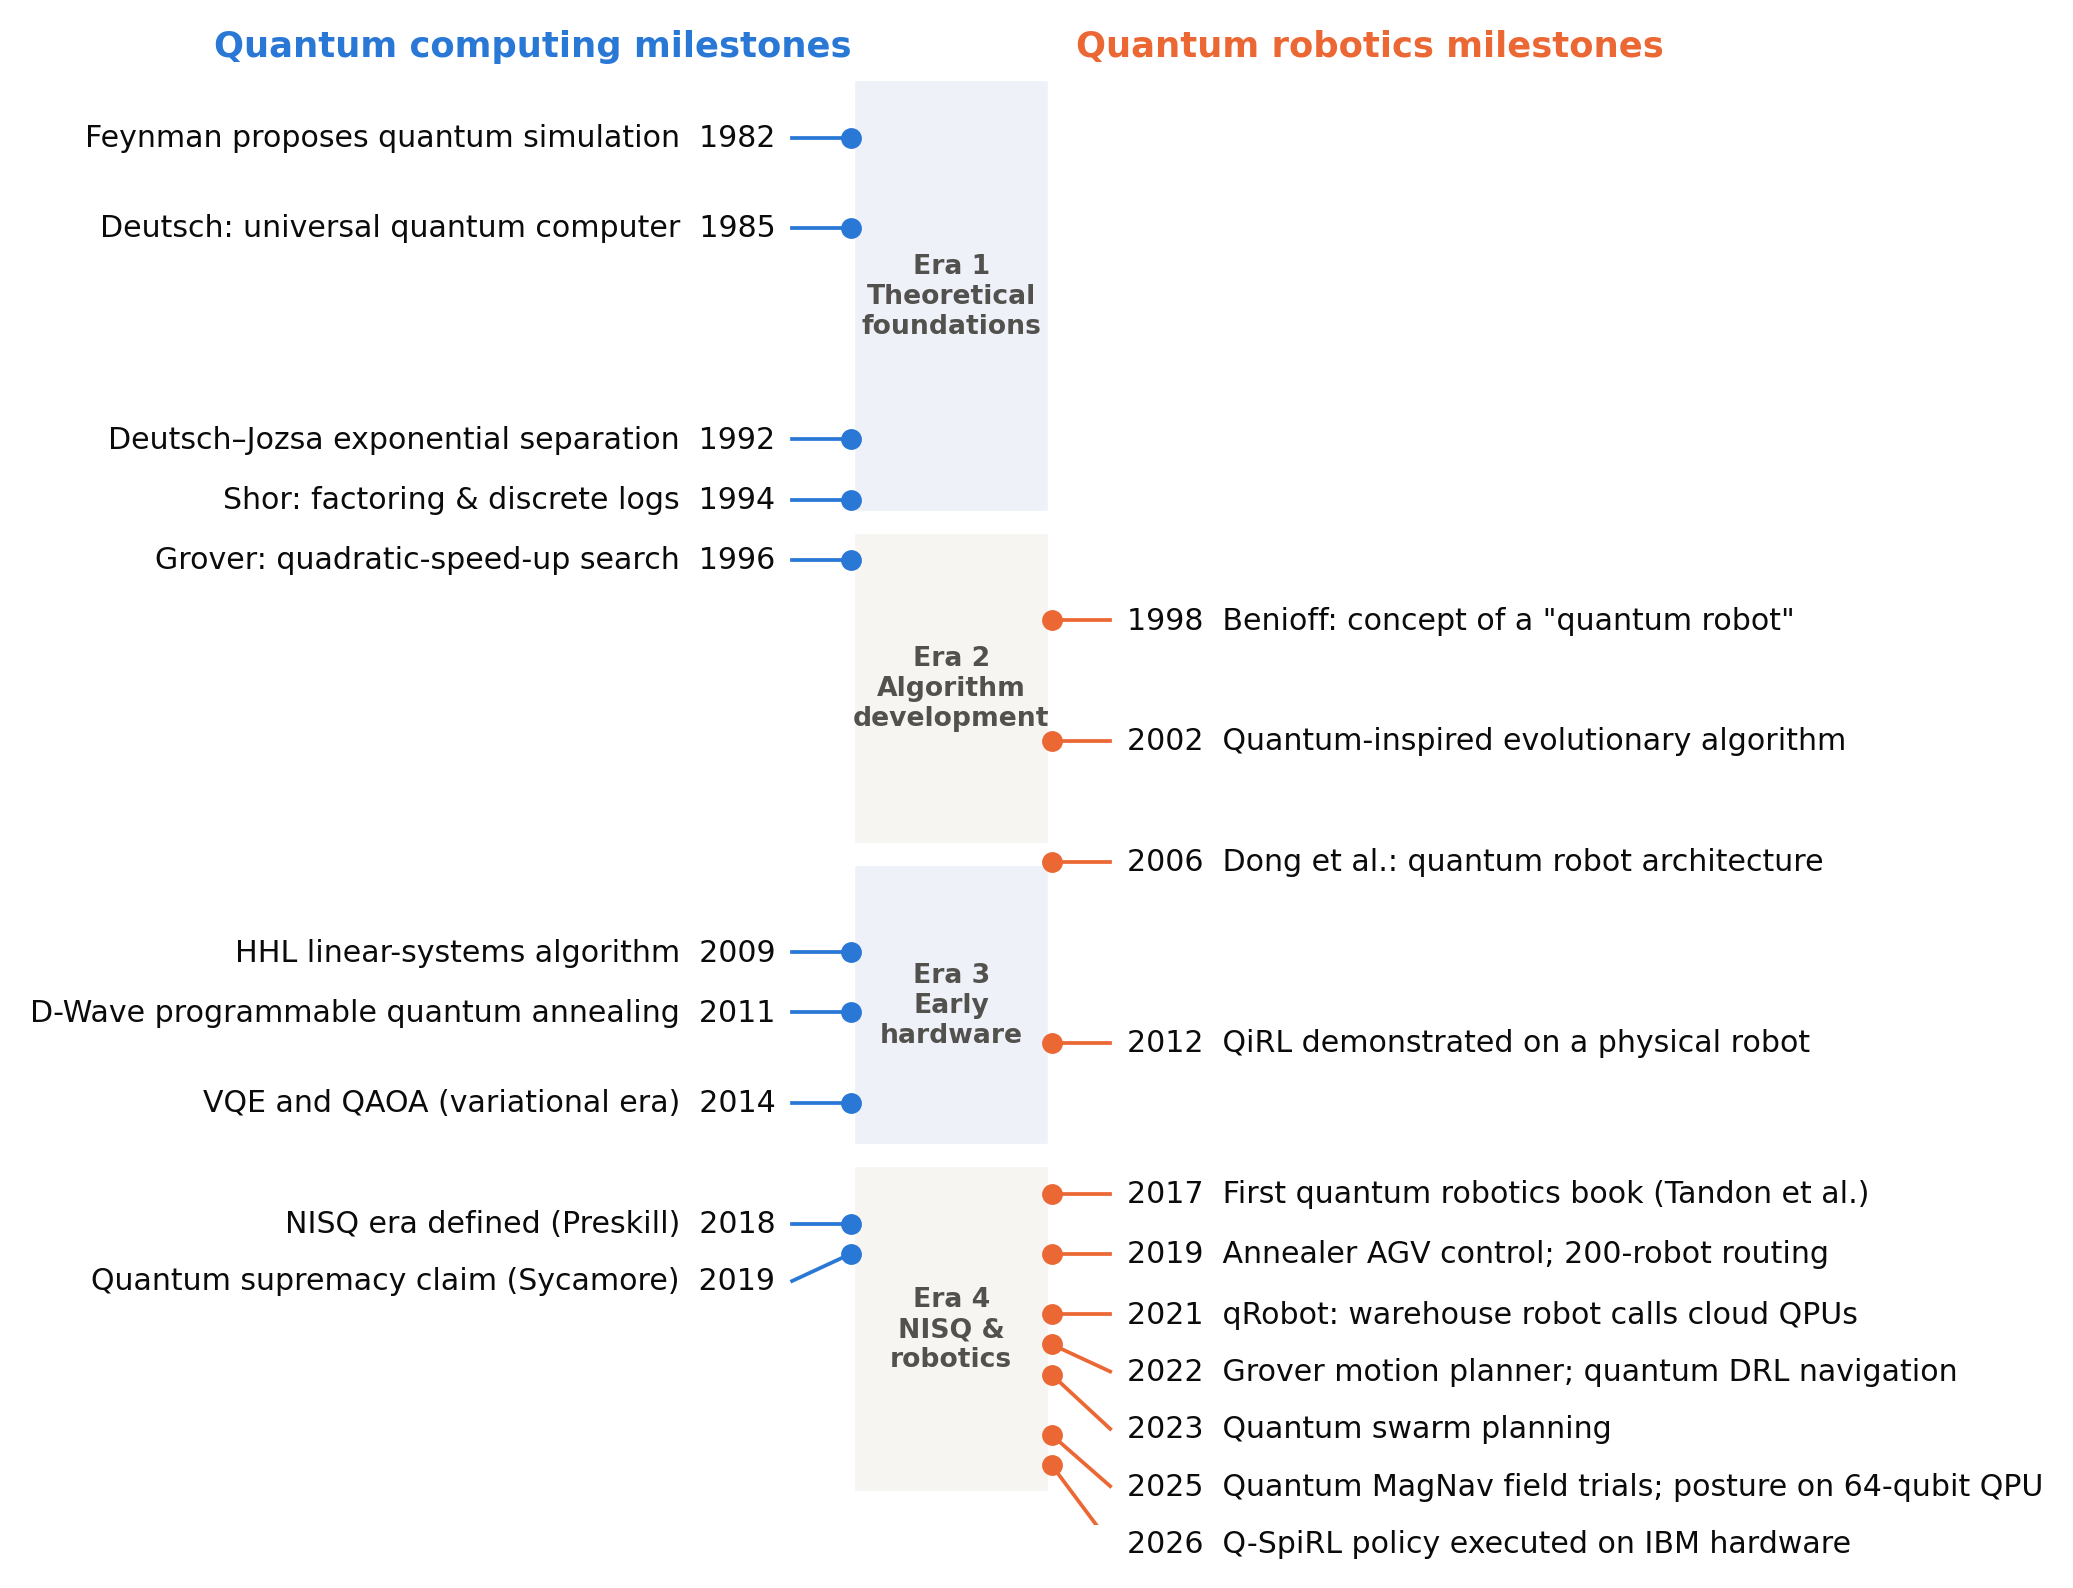
\includegraphics[width=\linewidth]{figures/fig3_timeline.png}
\caption{Evolution of quantum computing and quantum robotics, 1982--2026, across the four eras used in this survey. Robotics milestones are colored by technology: quantum computation, quantum-inspired classical computation, quantum sensing, and quantum communication.}
\Description{Vertical timeline from 1982 to 2026 with one row per year that has a milestone, shaded into four eras (theoretical foundations 1982 to 1993, algorithms 1994 to 2005, early hardware 2006 to 2015, NISQ 2016 onward). The left column lists quantum computing milestones from Feynman's 1982 proposal to below-threshold error correction in 2025; the right column lists robotics milestones, from Benioff's quantum robot in 1998 and quantum-inspired robot navigation in 2012 to annealer fleet routing, drone quantum communication, quantum magnetic navigation flights, and in 2026 a control agent running on a superconducting quantum processor.}
\label{fig:timeline}
\end{figure}


\section{Survey Methodology}\label{sec:method}
This survey follows the PRISMA 2020 reporting guideline~\cite{Page2021} and the systematic-review procedure of \citet{Kitchenham2007}; we report the PRISMA items that apply to a fast-moving computing literature and state in Section \ref{sec:selection} which record counts we cannot report.

\subsection{Research Questions}\label{sec:rqs}
The survey addresses five questions. \textbf{RQ1}: which quantum methods have been applied to which robotic functions (optimization and planning; learning, including quantum machine learning and reinforcement learning; sensing and communication; and decision-making and reasoning)? \textbf{RQ2}: what level of evidence supports each application, from theory to end-to-end deployment? \textbf{RQ3}: which reported benefits are genuinely quantum, and which come from quantum-inspired classical algorithms or are removed by dequantization? \textbf{RQ4}: which hardware and deployment constraints (qubit counts, noise, latency, quantum-classical communication, and size, weight, power, and cooling) limit quantum computing in robotics today? \textbf{RQ5}: which directions offer realistic benefit by 2030, and what is needed beyond?

\subsection{Search Strategy}\label{sec:search-strategy}
We searched IEEE Xplore, the ACM Digital Library, Scopus, Web of Science, SpringerLink, ScienceDirect, and arXiv (quant-ph, cs.RO, cs.LG), and followed the references of key papers and earlier surveys backward and forward~\cite{Petschnigg2019,Yan2024,Tandon2017,Meyer2022}. The core string combined a quantum block (e.g., ``quantum annealing'', QAOA, ``quantum reinforcement learning'', ``quantum-inspired'', ``quantum sensing'', ``quantum cognition''), a robotics block (e.g., robot*, ``autonomous vehicle*'', swarm, UAV, AGV, manipulator), and an application block (e.g., planning, navigation, localization, ``task allocation'', routing, control, learning, SLAM); a second string retrieved foundational reviews on NISQ algorithms, error mitigation, barren plateaus, fault tolerance, and dequantization. Because much of the work appears outside robotics venues, we also searched drones and UAVs, autonomous mobility and driving, control benchmarks such as the cart-pole, and automated storage and retrieval. The search covered 1982 onward; we closed the corpus in October 2026, and its most recent study was posted in August 2026. The strings for each database are in the supplementary material.

\subsection{Eligibility Criteria}\label{sec:criteria}
Studies were included if they (I1) proposed, evaluated, or reviewed a quantum or quantum-inspired method applied to a robotic function, (I2) provided algorithms, hardware, or theory on which such methods depend, or (I3) supplied the classical baselines needed for comparison. They were excluded if they (E1) used ``quantum'' only metaphorically, (E2) were not in English, (E3) duplicated an included study (the most complete version was kept, e.g., the journal version of \citet{Hohenfeld2024}), or (E4) addressed quantum communication without a robotic application. Studies meeting I1 are the \emph{primary studies}; those meeting only I2 or I3 are \emph{foundational works} and were not graded. Six quantum computer-vision studies without a robotic application fail I1 and are discussed, ungraded, in the supplementary material.

\subsection{Study Selection}\label{sec:selection}
We ran the searches iteratively, refining the strings as the scope settled, and screened candidates on title and abstract and then in full text. We did not log how many records each search returned or how many were excluded at each stage, so we cannot give the record counts of a complete PRISMA 2020 flow diagram; the diagram in the supplementary material shows the stages followed and the counts we can document. The corpus comprises 72 primary studies (65 empirical or theoretical studies and 7 reviews) and 107 foundational works. Figure \ref{fig:years} shows its growth. Before 2006 it holds only Benioff's two theoretical papers, since useful quantum algorithms had only just appeared and there was no hardware to run them; studies became regular once D-Wave annealers (2011) and cloud access to gate-based processors (2016) arrived, and 51 of the 72 appeared in 2023 or later, 25 in 2025 alone.

\begin{figure}[t]
\centering
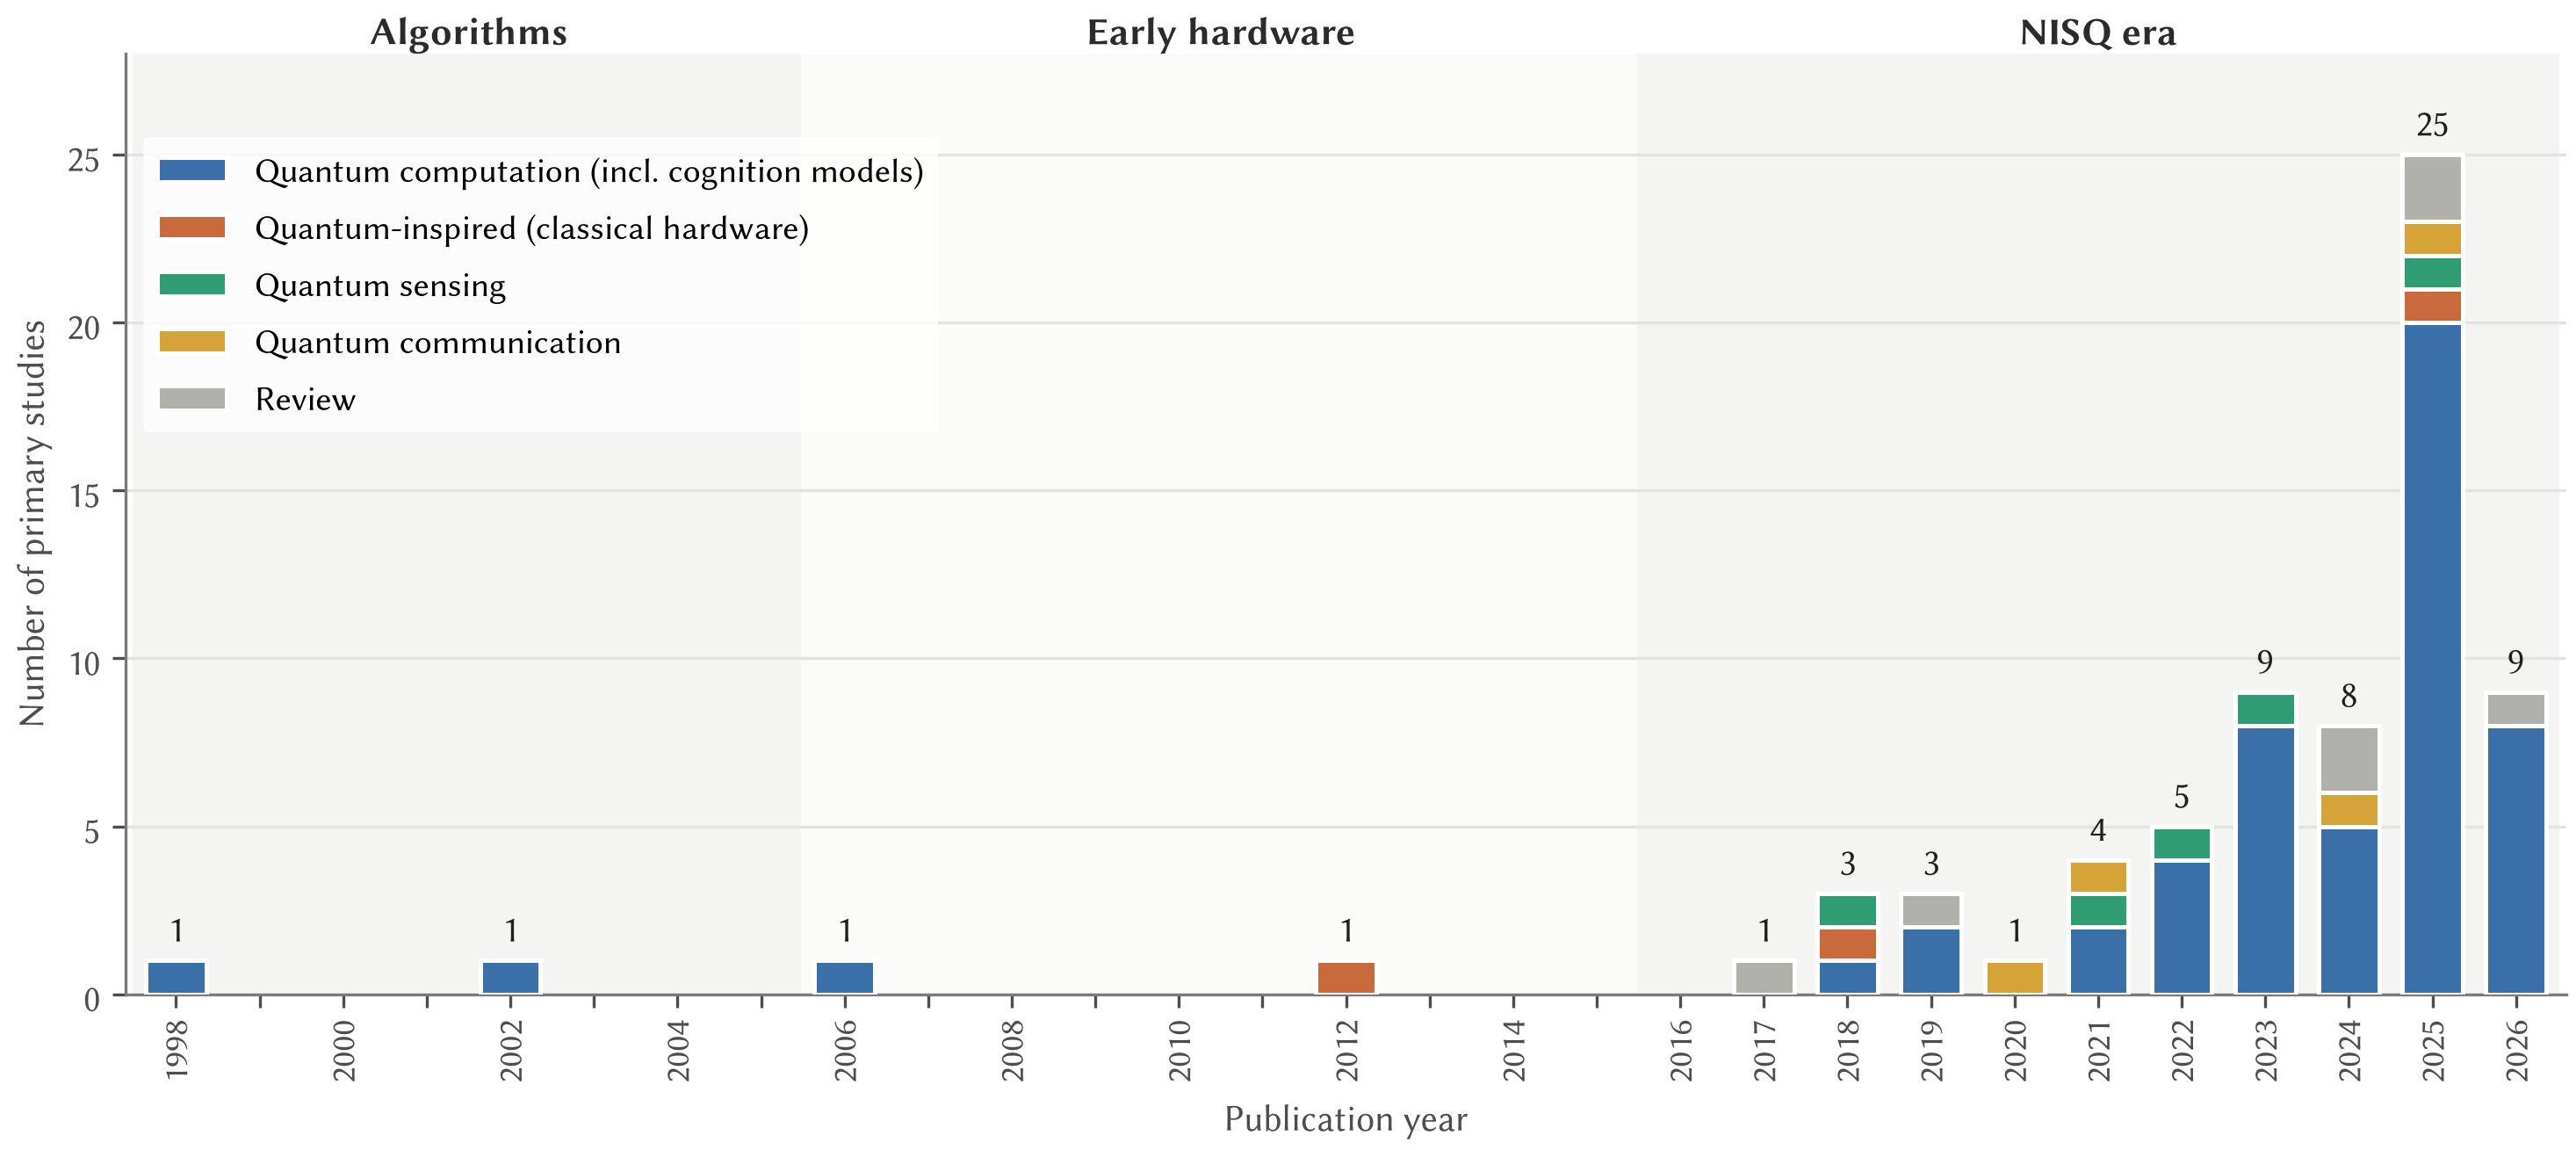
\includegraphics[width=0.92\linewidth]{figures/fig7_years.png}
\caption{Primary studies by publication year and technology type ($n=72$, including the 7 reviews), from the first quantum-robot paper in 1998 to 2026, with the eras of Figure~\ref{fig:timeline} shaded. The 2026 bar covers a partial year.}
\Description{Stacked bar chart with one bar per year from 1998 to 2026, shaded by era (algorithms, early hardware, NISQ). There is one study each in 1998, 2002, 2006, 2012, and 2017, and none in the other years before 2018; then 3 in 2018, 3 in 2019, 1 in 2020, 4 in 2021, 5 in 2022, 9 in 2023, 8 in 2024, 25 in 2025, and 9 in 2026. Quantum computation studies dominate from 2022 onward; quantum-inspired, sensing, communication, and review studies are spread thinly across the years.}
\label{fig:years}
\end{figure} When we retrieved the full texts, we checked every PDF against its bibliographic record. A few files turned out to be mislabeled or to carry wrong metadata, and we corrected these before extraction. All bibliographic records were then verified against publisher, DOI, or arXiv records.


\subsection{Data Extraction and Quality Assessment}\label{sec:extraction}
For each primary study we extracted the robotic task, quantum method and type, hardware or simulator, setup and baselines, key results, and stated and unstated limitations. Application studies were also appraised against seven criteria (problem formulation, classical baseline, experimental realism, hardware and noise reporting, performance metrics, reproducibility, and critical discussion), each judged not met, partly met, or met. We did not sum the judgments into a score, which would hide which criterion a study fails; the unmet criteria are reported as each study's principal limitation, and the per-study judgments are in the supplementary material. Three criteria fail most often: only 12 of the 59 appraised studies used a state-of-the-art classical baseline and 19 used none, only 6 were tested on a physical robot or in a realistic field setting, and of the 56 studies whose full texts we could check, only 14 released code or data. The first author screened the records, extracted the data, and assigned the levels, tags, and appraisal judgments; the second author reviewed them, and disagreements were resolved by discussion. Because the review was not independent grading, inter-rater agreement could not be measured (Section \ref{sec:validity}).

\subsection{Classification Scheme}\label{sec:classification}
\paragraph{Robotic-function taxonomy.} Each study was assigned to its primary function: \emph{optimization} (task allocation, routing, scheduling, kinematics), \emph{planning} (path, motion, and view planning, and localization posed as search), \emph{learning} (supervised and reinforcement learning), \emph{sensing and communication} (navigation sensors and quantum key distribution), or \emph{decision-making} (quantum-probability and cognitive models). Figure \ref{fig:taxonomy} shows the taxonomy, which structures Sections \ref{sec:opt} to \ref{sec:emerging}.

\begin{figure}[t]
\centering
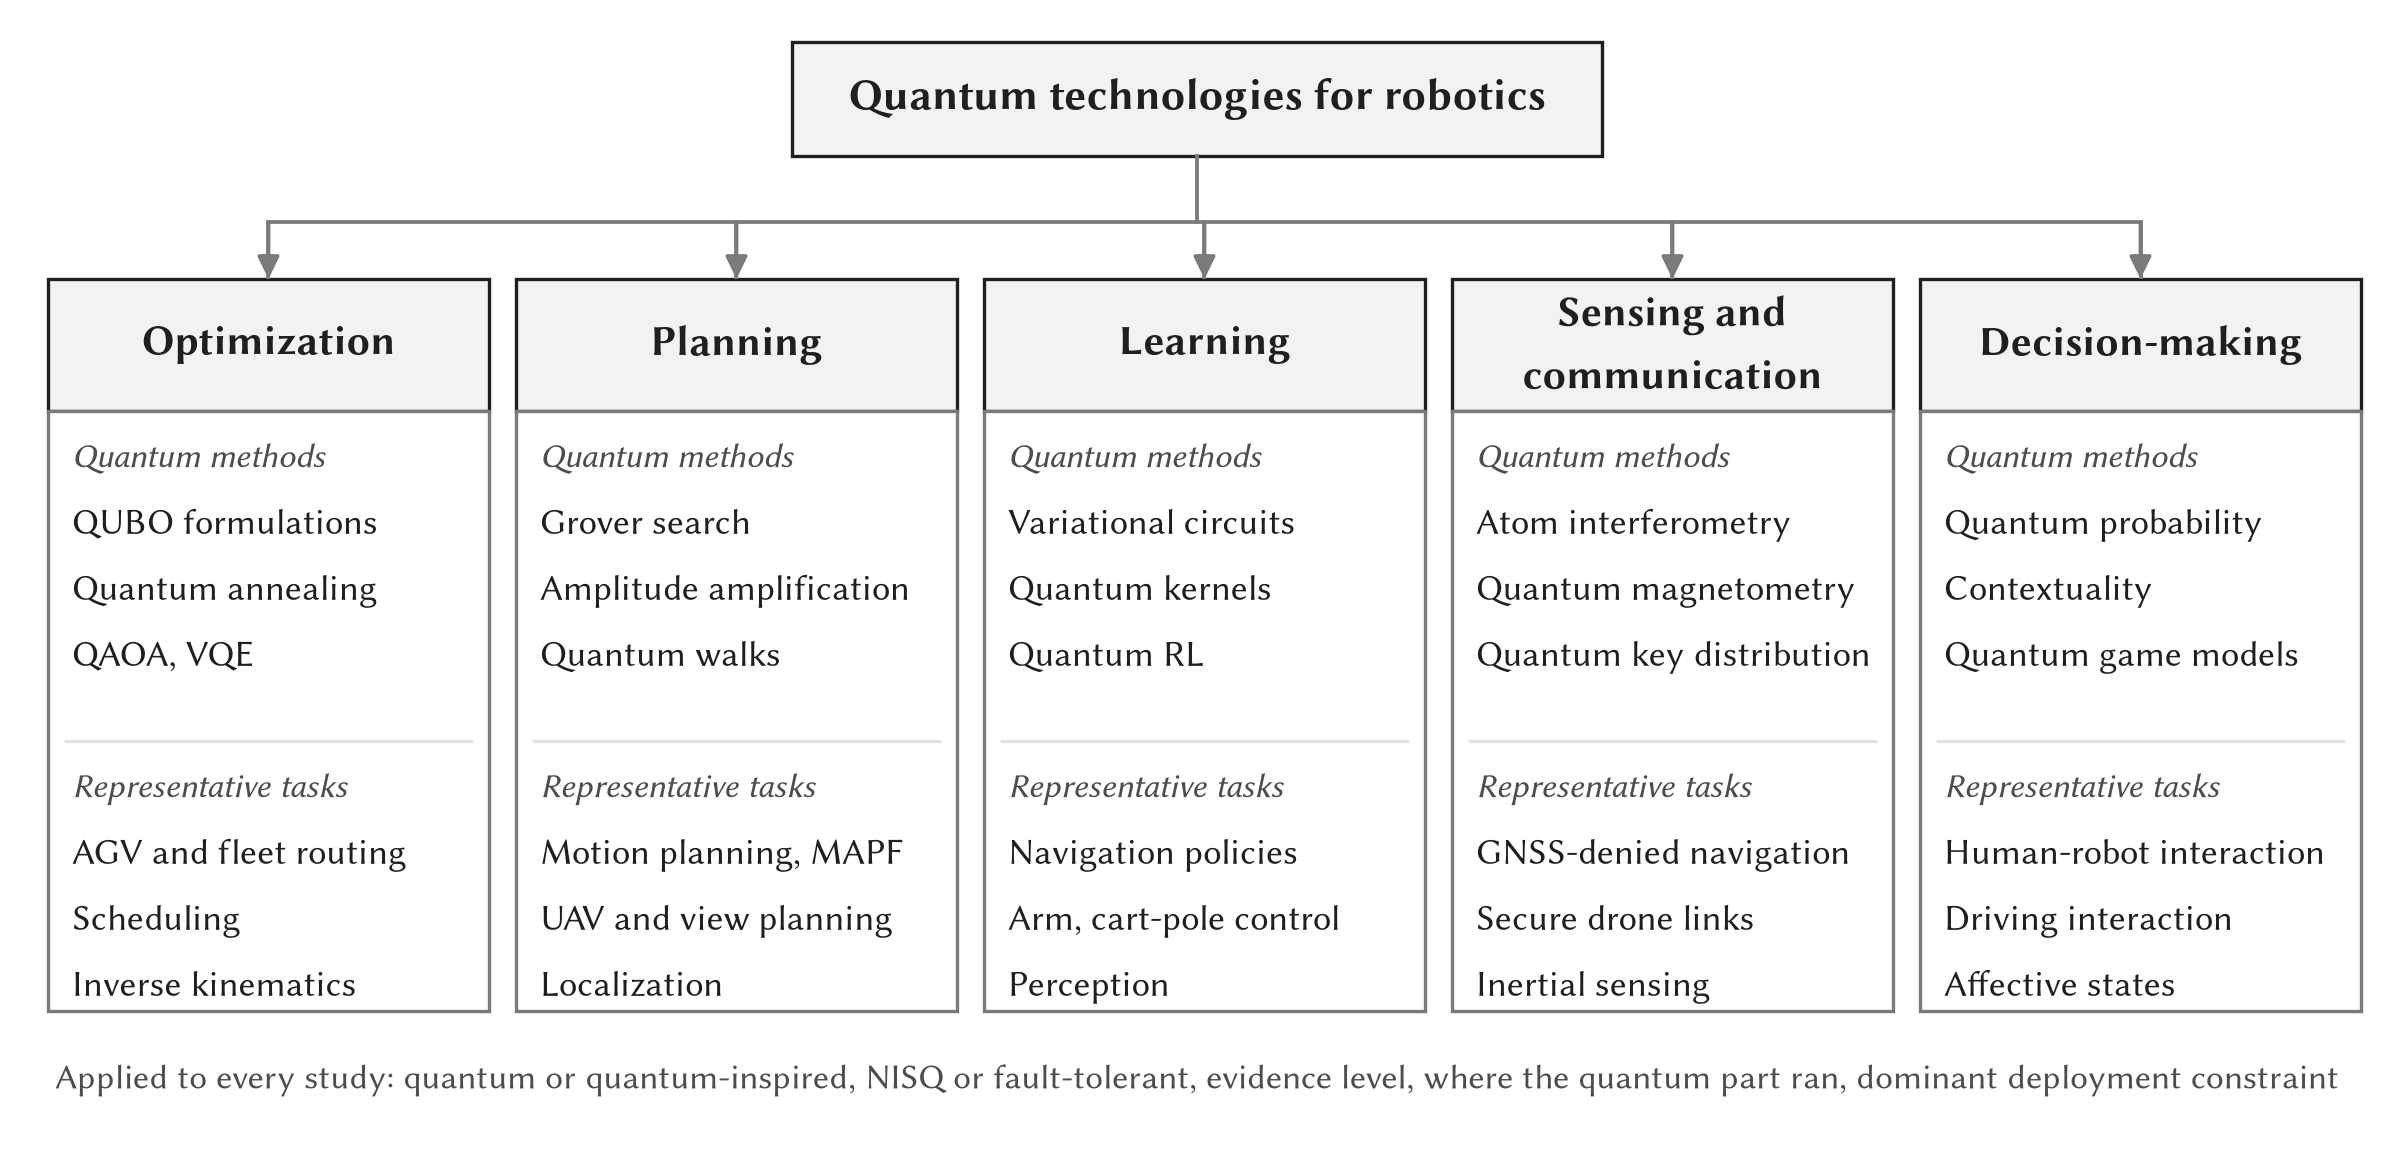
\includegraphics[width=1.00\linewidth]{figures/fig1_taxonomy.png}
\caption{Taxonomy of quantum technologies for robotics: robotic functions (top), the quantum methods applied to each (middle), and representative robotic tasks (bottom).}
\Description{Tree diagram with ``Quantum technologies for robotics'' at the root and five branches (optimization, planning, learning, sensing and communication, decision-making); each branch lists quantum methods such as QUBO and annealing, QAOA, Grover search, variational circuits, quantum sensors, and quantum-probability models, and example tasks such as AGV routing, path planning, robot navigation RL, GNSS-denied navigation, and human-robot interaction.}
\label{fig:taxonomy}
\end{figure}

\paragraph{Evidence hierarchy.}
Evidence was graded on six ordered levels (Table \ref{tab:levels}), separating what has been argued (L1), simulated (L2), executed on quantum hardware (L3), coupled to a robot or robot simulator in a closed loop (L4), demonstrated on a physical robot or vehicle (L5), and deployed end to end with a measured advantage over a classical baseline (L6). A study's level is the highest reached by its own experiments.

\paragraph{Quantum-execution tag.} The levels grade integration with a robot, not whether the quantum part ran on quantum hardware: a study can couple a \emph{simulated} circuit to a simulated robot and reach L4 without a quantum processor. Every study therefore also carries an execution tag: \emph{none}, \emph{simulated}, \emph{QPU} (at least partly run on a gate-based processor or annealer), \emph{quantum sensor or link hardware}, or \emph{classical} (quantum-inspired). Level and tag are read together, e.g., L4/simulated (Table \ref{tab:execution}). We kept one ordered scale rather than two axes because the first question a roboticist asks is how close a result is to a working robot; the cost is that the levels do not rank quantum evidence, so we compare studies on both dimensions. Studies were also classified by method family, hardware, regime (NISQ or fault-tolerant), and dominant deployment constraint; these codes are in the dataset.

\begin{table}[t]
\caption{Evidence hierarchy used to grade the primary studies, with the number of studies at each level (65 studies; 7 reviews excluded).}
\label{tab:levels}
\footnotesize
\begin{tabular}{@{}>{\raggedright\arraybackslash}p{0.060\dimexpr\linewidth-10\tabcolsep\relax}>{\raggedright\arraybackslash}p{0.160\dimexpr\linewidth-10\tabcolsep\relax}>{\raggedright\arraybackslash}p{0.420\dimexpr\linewidth-10\tabcolsep\relax}>{\raggedright\arraybackslash}p{0.050\dimexpr\linewidth-10\tabcolsep\relax}>{\raggedright\arraybackslash}p{0.310\dimexpr\linewidth-10\tabcolsep\relax}@{}}
\toprule
\textbf{Level} & \textbf{Name} & \textbf{Definition} & \textbf{n} & \textbf{Examples} \\ \midrule
L1 & Theoretical & Analysis, complexity argument, or conceptual model only & 6 & \cite{Benioff1998,Lawless2023,Humr2025} \\
L2 & Simulation & Quantum circuits or annealing simulated on classical computers & 19 & \cite{Chella2022,Lathrop2023,Roh2025} \\
L3 & QPU experiment & At least part of the method executed on real quantum hardware & 23 & \cite{Clark2019,Leib2023,Otani2025} \\
L4 & Robot-in-the-loop & Quantum computation coupled in a closed loop to a robot or high-fidelity robot simulator & 10 & \cite{Hohenfeld2024,Sinha2023,Quang2025} \\
L5 & Physical demonstration & Behavior demonstrated on a physical robot, vehicle, or mechanical control system & 6 & \cite{Dong2012,Liu2021,Sun2025} \\
L6 & End-to-end deployment & Field operation in a realistic setting with a measured advantage over a classical baseline & 1 & \cite{Muradoglu2025} \\
\bottomrule
\end{tabular}
\end{table}



\subsection{Threats to Validity}\label{sec:validity}
\emph{Coverage}: the field moves quickly, its terminology is loose (``quantum'', ``quantum-inspired'', and ``quantum-like'' are used interchangeably), and several key results are preprints~\cite{Altrabulsi2026,Muradoglu2025}; broad strings, seven databases, and reference chasing reduce but do not remove the risk, and non-English and unpublished industrial work is missing. \emph{Publication bias} probably favors positive results. \emph{Classification}: levels were assigned from what was reported, which is often incomplete on hardware, shots, and latency; when in doubt, we assigned the lower level. \emph{Selection and grading}: one reviewer screened and extracted, stage counts were not logged, and the levels were reviewed rather than independently assigned by the second author, so neither search completeness nor grading reliability can be measured; every judgment is published in the supplementary material and dataset so readers can check it. \emph{Synthesis}: heterogeneous tasks, metrics, and baselines prevented a meta-analysis, so the synthesis is narrative. \emph{Recency}: 16 primary studies were preprints when graded and 34 appeared in 2025 or 2026; the levels describe the record at the time of our search, not the limits of the technologies.

\section{Quantum Optimization for Robot Coordination, Scheduling, and Kinematics}\label{sec:opt}

\subsection{Methods}\label{sec:opt-methods}
Most robotic optimization problems are first written as QUBO or Ising models (Section \ref{sec:qc}); \citet{Lucas2014} catalogued such formulations for the traveling-salesman, coloring, and scheduling problems that underlie routing and task allocation. A QUBO can be solved by annealing~\cite{Johnson2011} or by QAOA~\cite{Farhi2014}, whose quality improves with depth $p$ but whose single-layer guarantee on 3-regular MaxCut (0.6924) is weaker than that of the best classical algorithms. Constraint-preserving mixers enforce hard constraints without penalty terms~\cite{Hadfield2019}, optimal parameters follow transferable patterns~\cite{Zhou2020}, and optimizing the conditional value-at-risk of the samples improves convergence~\cite{Barkoutsos2020}. Annealers were tried on robot-like planning early: \citet{Rieffel2015} found that the mapping, the embedding, and the annealing schedule all strongly affect performance, \citet{Neukart2017} redistributed cars across a congested road network, and \citet{Yarkoni2022} review industrial uses. No exponential speed-up is proven for NP-hard optimization, and \citet{Guerreschi2019} estimated that a runtime crossover for QAOA would need several hundred to a few thousand qubits; the realistic benefit for robotics is faster good-enough solutions to large allocation and routing problems.

\subsection{Multi-Robot Fleets and Automated Guided Vehicles}\label{sec:opt-fleets}
Fleets of AGVs and transport robots form the largest and most hardware-tested cluster of studies. \citet{Ohzeki2019} formulated collision-free AGV control in a DENSO plant as a QUBO that selects one candidate route per vehicle, with penalties for conflicting road use, re-solved in every period (supplementary Figure S2). With 10 AGVs, D-Wave 2000Q returned plans quickly but handled only small instances (at most 60 variables) and needed post-processing to repair infeasible samples, whereas the Fujitsu Digital Annealer and Gurobi handled larger problems; the formulation, not the quantum hardware, delivered most of the benefit. \citet{Quang2025} scaled the approach to a commercial AGV operating system: candidate-route generation cut the variables by 78--96\% and dynamic clustering kept sub-QUBOs below 10,000 variables, so that a simulated fleet of up to 1,000 AGVs on real warehouse data could be routed on D-Wave hardware or classical solvers. It is the largest robotics application of annealing we found, but its gains come mostly from decomposition, and it does not show the annealer beating classical solvers on the same subproblems. \citet{Clark2019} produced valid conflict-free routes for up to 200 robots on a D-Wave 2000Q, although ``real time'' referred to the anneal, not to the end-to-end latency with cloud access and embedding~\cite{Ravi2021}.

Three studies compared solvers head to head. \citet{Smierzchalski2024} solved AGV scheduling with up to 21 vehicles on D-Wave's hybrid solvers in seconds, comparable to CPLEX, but note that the proprietary hybrid solver hides the QPU's contribution, a caveat for much of this literature. \citet{Leib2023}, in one of the most rigorous comparisons, scheduled transport robots in a BASF laboratory: Gurobi reached comparable quality 10 to 100 times faster on smaller instances, the Fujitsu hybrid led on the largest, and D-Wave showed limited promise, so the practical benefit came from quantum-inspired hardware. qRobot~\cite{AtchadeAdelomou2021} dispatched a warehouse robot's routing QUBOs from a Raspberry Pi to cloud back ends, a useful architecture tested only on very small instances, and \citet{Windmann2023} scheduled storage-and-retrieval jobs with QAOA on an IBM processor, where again only small instances fit.

\subsection{Industrial Trajectories, Assembly, and Inspection}\label{sec:opt-industrial}
\citet{Schuetz2022} sequenced robot tasks in BMW body and paint shops with a classical genetic algorithm that beat greedy baselines on industry-scale data, testing annealing only as a plug-in; the paper is candid that the performance is classical. \citet{Willmann2025} balanced a small assembly line on a D-Wave Advantage 4.1: the annealer found optimal configurations, but the full workflow took about 10,110 s against 0.03 s for an exact classical solver, a rare and useful measurement of how overheads outside the anneal dominate. \citet{Osaba2025} planned inspection-robot trajectories with D-Wave's hybrid solvers and reported quality competitive with Gurobi and OR-Tools at lower computation time on five industrial cases, one of the few runtime benefits reported, which we treat as preliminary given the short paper and proprietary solver.

\subsection{Kinematics}\label{sec:opt-kinematics}
\citet{Otani2025} encoded each link of a two-link manipulator in a qubit, with entangling gates representing parent-child coupling, and found on the 64-qubit RIKEN/Fujitsu computer that entanglement reduced positioning error compared with an unentangled circuit; with two qubits and no comparison to standard inverse-kinematics (IK) solvers, it is a hardware demonstration, not evidence of advantage. \citet{Salloum2026} discretized planar IK into a QUBO, compared embeddings on D-Wave's Pegasus and Zephyr topologies, and reached lower time-to-solution than classical QUBO baselines on larger instances, while stating that the method does not beat continuous IK solvers. Kinematics can thus run on today's hardware only in discretized or toy form.

\subsection{Assessment}\label{sec:opt-assessment}
Current QUBO formulations represent continuous robot problems only after coarse discretization, whereas sampling-based planners~\cite{LaValle1998,Karaman2011} and task-and-motion planners~\cite{Garrett2021} handle them directly. Where mature solvers were compared, the picture is consistent: Gurobi or CPLEX matched or beat the annealer on small and medium instances~\cite{Ohzeki2019,Smierzchalski2024,Leib2023}, an exact solver was orders of magnitude faster end to end~\cite{Willmann2025}, and advantages on the largest instances came from quantum-inspired digital annealers~\cite{Leib2023,Goto2019}. Evidence reaches L3, and L4 in simulation for fleet routing~\cite{Quang2025}; no study reports a robust advantage over the best classical solver, and one short study's runtime gain awaits confirmation~\cite{Osaba2025}. Penalty-based QUBOs inflate qubit counts and sparse connectivity forces embedding overheads, so most of the benefit comes from formulating the problem well, not from quantum hardware.

\section{Quantum Search for Planning, Navigation, and Localization}\label{sec:search}

\subsection{Methods}\label{sec:search-methods}
Grover's algorithm finds a marked item among $N$ with $O(\sqrt{N})$ oracle calls~\cite{Grover1996}; amplitude amplification generalizes it~\cite{Brassard2002}, and amplitude estimation gives a near-quadratic speed-up for Monte Carlo estimation~\cite{Montanaro2015}, relevant to particle-filter localization~\cite{Dellaert1999}. Quantum walks speed up search and agent deliberation~\cite{Paparo2014}, and coherent distance estimation reduces queries for nearest-neighbor methods~\cite{Wiebe2015}. These speed-ups count oracle queries, not wall-clock time, and need fault-tolerant hardware; \citet{Benioff2002} had already shown that a quantum robot gains nothing from Grover search when it must move through the region it searches.

\subsection{Motion Planning and Swarm Planning}\label{sec:search-planning}
\citet{Chella2022} encoded the tree of a robot's possible action sequences in a reversible Boolean oracle so that Grover search finds a goal-reaching plan with $O(\sqrt{N})$ oracle calls. The noiseless Qiskit simulations were limited to about 27 qubits, qubit counts grow with plan depth, the oracle assumes a known map, and there is no comparison with A* or sampling-based planners. \citet{Chella2023} extended the planner to small simulated swarms, which reached a target faster than generic ant-colony simulations. \citet{Lathrop2023} came closest to the planners robots use: they recast sampling-based planning as a database-oracle problem, and in a classical simulation their quantum RRT showed the expected quadratic speed-up over classical RRT, a gain that only fault-tolerant hardware would make real. \citet{Nigatu2025} built the Grover oracle from a circuit trained to approximate manipulator kinematics and reported simulated speed-ups of up to 93 times over classical optimizers, and \citet{Sarkar2024} reached tours within about 7\% of OR-Tools optima with a simulated quantum ant-colony method whose accuracy fell as qubits grew. All rest on Grover's query advantage; supplementary Figure S3 shows their shared structure.

\subsection{Multi-Agent Pathfinding and UAV Navigation}\label{sec:search-mapf}
\citet{Gerlach2025} gave the first optimal hybrid algorithms for multi-agent pathfinding (MAPF): branch-and-cut-and-price decomposes agent conflicts into small QUBO subproblems, solved by a quantum or quantum-inspired solver, and on standard benchmarks, including runs on a D-Wave Advantage, the approach compared favorably with state-of-the-art MAPF solvers. It is methodologically the strongest multi-robot result in the corpus, because the quantum part sits inside a provably optimal framework with strong baselines. \citet{GonzalezVillasmil2026} solved multi-robot paths on grids of up to $10\times 10$ cells as one QUBO, with near-optimal results but classical planners faster at every size, and \citet{Rao2024} designed a constraint-preserving QAOA~\cite{Hadfield2019} for coverage planning against a weak depth-first baseline. For drones, QUAV~\cite{Innan2025} produced feasible QAOA trajectories on IBM's ibm\_kyiv processor for small graphs without a classical benchmark; \citet{OsabaDrone2025} combined QAOA clustering with annealer routing, with the quantum share not isolated; and \citet{Bang2026} turned language instructions into constraint-preserving CVaR-QAOA for multi-drone assignment, recovering the optimum in 96.3\% of cases in statevector simulation.

\subsection{Perception-Driven Planning and Localization}\label{sec:search-loc}
HQC-NBV~\cite{Yu2025} encoded next-best-view selection in a Hamiltonian and explored simulated scenes 7.9--49.2\% more efficiently than classical approaches, with simulated circuits and weak baselines. \citet{Antero2025} posed localization on a known map as a Grover search for the cell whose stored pattern matches the robot's sensor view, needing $O(\sqrt{N})$ queries instead of the $O(N)$ evaluations of grid-based Monte Carlo localization. It localized correctly in simulation and on cloud hardware, but accuracy fell as maps grew; the speed-up is an asymptotic query count, and Section \ref{sec:resource} estimates what it would cost on a fault-tolerant machine.

\paragraph{Evidence level.} Grover-based planning remains at L2~\cite{Chella2022,Nigatu2025}; QAOA drone planning~\cite{Innan2025} and Grover localization~\cite{Antero2025} reach L3 on very small problems, and hybrid MAPF reaches L3 with strong baselines~\cite{Gerlach2025}. Apart from the last, no study compares against A* or RRT*~\cite{Karaman2011}, or against Monte Carlo localization on realistic maps. The obstacle is the oracle: building it for a map or plan tree needs many ancilla qubits and deep circuits, and the quadratic gain is quickly consumed by error-correction overheads~\cite{Fowler2012}.

\section{Quantum Learning for Robots}\label{sec:learning}

\subsection{Supervised Quantum Machine Learning}\label{sec:qml}
Quantum machine learning (QML) has developed along two lines~\cite{Biamonte2017,Schuld2021,Wang2024}: fault-tolerant linear algebra, such as quantum clustering~\cite{Lloyd2014} and support vector machines~\cite{Rebentrost2014} that assume quantum random-access memory (qRAM), and NISQ parameterized circuits trained classically~\cite{Mitarai2018,Farhi2018}, with data encoding read as a feature map~\cite{Schuld2019}. Hardware classifiers reached 100\% accuracy on synthetic data suited to their feature map~\cite{Havlicek2019}, and quanvolutional networks showed no advantage over random classical features~\cite{Henderson2020}. Applications to robot perception are surprisingly scarce. \citet{Roh2025} used a fast quantum convolution for object detection on the KITTI driving dataset, with simulated circuits but real data, and candidate applications in object recognition and sensor fusion~\cite{Petschnigg2019,Yan2024} face the fact that quantum image representations handle two-dimensional images, whereas robots mostly see three-dimensional point clouds. The first QML study on real industrial robot data, with PAL Robotics, built a test oracle for regression testing whose prediction error was about 15\% lower than a classical network's~\cite{Wang2025}, pointing to offline software assurance as a latency-tolerant niche. Earlier, \citet{Goncalves2018} ran small quantum neural networks on IBM's five-qubit processor for a quantum robot~\cite{Benioff1998}.

\paragraph{Barren plateaus and dequantization.} Gradients of randomly initialized circuits vanish exponentially with the number of qubits~\cite{McClean2018}, global costs cause barren plateaus even at shallow depth~\cite{Cerezo2021b}, and architectures provably free of them may be classically simulable~\cite{Larocca2025}; robot learning, with high-dimensional inputs and global rewards, runs straight into this limit. Several claimed exponential QML speed-ups have also been matched classically under the same input assumptions~\cite{Tang2019,Chia2020}, and their fine print rarely holds for robot data~\cite{Aaronson2015}.

\subsection{Quantum Reinforcement Learning}\label{sec:qrl}
Quantum reinforcement learning (QRL) has three strands~\cite{Meyer2022,Dunjko2018}: quantum-inspired action selection by Grover-like amplification~\cite{Dong2008}, quantum-walk speed-ups of agent deliberation~\cite{Briegel2012,Paparo2014}, and, now dominant, variational quantum circuits (VQCs) in place of the networks of deep RL~\cite{Sutton2018}, with VQC Q-learning~\cite{Chen2020,Skolik2022}, policy gradients with a learning separation on artificial tasks~\cite{Jerbi2021}, evolutionary training~\cite{Chen2022}, and multi-agent QRL~\cite{Yun2022}. Circuit design largely decides whether such agents learn continuous control at all~\cite{Kruse2024}; supplementary Figure S4 shows the common template.

\paragraph{Navigation and control.} The quantum-inspired QiRL of \citet{Dong2012} learned obstacle avoidance faster than temporal-difference learning in simulation and on a real two-wheeled robot, on classical hardware and against a basic baseline. Variational circuits replaced the Q-network of a simulated Turtlebot~\cite{Hohenfeld2024}: they learned optimal policies with far fewer parameters and beat equal-sized classical networks, but a full-size classical network trained faster and did better in a dynamic environment. With continuous actions~\cite{Dragan2025}, an 851-parameter quantum model solved small mazes in all trials but the largest in only 10 of 30, whereas a 136,451-parameter classical model solved all. Nav-Q~\cite{Sinha2023} used a quantum critic only in training for self-driving navigation in CARLA and trained more stably, although noise degraded training; a fully quantum Soft Actor-Critic controlled a simulated arm with about 100 times fewer parameters than the classical agent~\cite{Acuto2022}; and a 17-qubit version on Walker2d beat a classical SAC by about 8\% with 41 instead of 1,250 parameters~\cite{Lokossou2025}. Multi-agent QRL with quantum critics coordinated simulated UAV fleets and autonomous mobility~\cite{Park2023,Park2024}, and quantum-spiking hybrids reached up to 99\% success in grid worlds, with a policy run on IBM hardware~\cite{Altrabulsi2026}, or fewer safety violations for simulated drones~\cite{Taghavi2025}.

\paragraph{Real-time control.} Two studies take quantum policies out of simulation. \citet{Sun2025} balanced a physical cart-pole with a variational policy, but only because the circuit was simulated locally: on a cloud QPU each decision took over 3.7 s. \citet{Ngo2026} kept the QPU: a single-qubit agent ran on the VTT Q5 processor, and programming its readout electronics directly made execution more than ten times faster, up to 6.2 inference steps per second, still short of the tens of hertz a control loop needs. Together they are the first measurements of what it would take to put a QPU inside a control loop.

\subsection{Assessment}\label{sec:learning-assessment}
QRL's one consistent advantage is \emph{parameter efficiency}: quantum policies reach comparable returns with one to two orders of magnitude fewer trainable parameters~\cite{Hohenfeld2024,Acuto2022,Dragan2025,Lokossou2025}. Adequately sized classical networks still train faster and do better in the hardest environments~\cite{Hohenfeld2024,Dragan2025}, a formal advantage exists only for artificial tasks~\cite{Jerbi2021}, and a smaller parameter count is not shorter training, better sample efficiency, or lower energy. Supervised QML for robots is at L1--L2; variational QRL reaches L4 only with simulated robots and noise-free circuits; Q-SpiRL and the VTT agent reach L3 on hardware~\cite{Altrabulsi2026,Ngo2026}; and at L5 sit the quantum-inspired QiRL~\cite{Dong2012} and the locally simulated cart-pole policy~\cite{Sun2025}, the only genuinely quantum method to reach a physical system. What really limits robot RL is the cost of real-world samples~\cite{Kober2013}, and no QRL study shows better sample efficiency on a robot task; training on real QPUs would also mean millions of circuit evaluations, each facing cloud queueing (Section \ref{sec:hybrid}).

\section{Quantum Sensing and Communication for Mobile Robots}\label{sec:sensing}

\subsection{Quantum Navigation Sensors}\label{sec:sensors}
Quantum sensing uses quantum systems, such as cold atoms, nitrogen-vacancy (NV) centers, and trapped ions, to measure physical quantities with sensitivity and stability beyond those of classical sensors~\cite{Degen2017}. Cold-atom interferometers provide accelerometers and gyroscopes with extremely low bias drift, and optically pumped magnetometers measure weak magnetic fields. \citet{Bongs2019} reviewed the transition of atom-interferometric sensors from the laboratory to the field and identified SWaP-C, dynamic range, and robustness as the main engineering barriers.

\citet{Cheiney2018} addressed the main obstacles to using cold-atom interferometers for navigation, namely their low sample rate and limited dynamic range. In their hybrid accelerometer, a matter-wave interferometer, which is extremely stable but slow, continuously estimates the bias drift of a fast classical accelerometer through a Kalman filter. Under experimentally simulated vehicle-like conditions, the hybrid sensor combined a 400 Hz bandwidth with a stability of 10 ng after 11 hours of integration. \citet{Wang2021} approached the same problem with maximum-likelihood fusion. A co-located classical accelerometer resolves the phase wrapping of the quantum sensor, and the recovered quantum measurement in turn recalibrates the bias of the classical sensor. In a simulated one-dimensional inertial-navigation scenario, this reduced the navigation error. \citet{Wang2023} assessed NV-center (quantum diamond) magnetometers as aids to inertial navigation where global navigation satellite systems (GNSS) are unavailable, They combined simulated magnetic measurements with probabilistic data association and Viterbi map-matching to estimate the navigation errors that current and near-term sensitivities would allow. These solid-state sensors could eventually be small enough for mobile robots. Atom interferometers have also left the laboratory. \citet{Geiger2011} operated a matter-wave accelerometer on board an aircraft, and \citet{Templier2022} built the first hybrid three-axis quantum accelerometer, which tracks the full acceleration vector at 1~kHz with a 50-fold stability gain over its classical triad and no longer needs to be aligned with a predefined axis.

\citet{Muradoglu2025} demonstrated ``quantum-assured'' magnetic-anomaly navigation, in which quantum magnetometers measure the Earth's crustal magnetic field and a denoising and map-matching suite compares the measurements with anomaly maps to provide passive, jamming-resistant position fixes without GNSS. In flight trials on a crewed aircraft (a Cessna 208B) from ground level to about 19,000 ft, the system achieved up to about 46 times lower positioning error than a velocity-aided strategic-grade inertial navigation system (INS), with the best final error of 22 m (0.006\% of the distance flown) and at least an 11-fold advantage in every airborne trial. On a ground vehicle with public maps, the error was about 7 times lower than that of the INS. The system learns vehicle-specific parameters online and is compact enough for fixed-wing drones. This is the strongest field evidence we found that quantum technology already improves a robotic capability. Two qualifications apply: the benefit comes from quantum sensing, not quantum computing, and the result is a company-led preprint that still needs independent replication.


\subsection{Quantum Communication between Robots}\label{sec:qkd}
\citet{Khoshnoud2020}, with NASA JPL, implemented single-photon generation by spontaneous parametric down-conversion, polarization encoding, and single-photon detection on networks of aerial and ground robots, as a step toward quantum-secured and entanglement-assisted multi-robot coordination. \citet{Tian2023} reported drone-based quantum key distribution (QKD): a compact, polarization-encoded decoy-state BB84 transmitter on an octocopter distributed secret keys in real time over 200 m at an average rate of 8.48 kHz. \citet{Liu2021} distributed entangled photons over 1~km, with one drone carrying the entangled-photon source and a second drone acting as an optical relay, and still violated the CHSH inequality ($S=2.59\pm 0.11$). \citet{Conrad2025} built a modular, reduced-SWaP QKD transmitter and receiver and demonstrated drone-to-drone, drone-to-vehicle, and vehicle-to-vehicle quantum communication with finite-key secure rates of 1.6--20 kbps, supported by device models of the non-idealities of mobile operation. Quantum-secured links between moving robots have thus reached field demonstration. That puts them on a par with quantum navigation sensing and well ahead of quantum computation for robots.

Of all the branches covered here, this one is the most mature. On the strength of one company-led preprint, magnetic-anomaly navigation reaches L6, with end-to-end field operation on aircraft and a ground vehicle and a measured advantage over a strategic-grade INS~\cite{Muradoglu2025}, and QKD and entanglement distribution between drones and vehicles reach L5~\cite{Tian2023,Conrad2025,Liu2021}.

What limits it now is mostly engineering: size, weight, power, and cost, together with dynamic range. Cold-atom sensors are still bulky, power-hungry, and limited in bandwidth, and they must be fused with classical sensors by Kalman-type estimators~\cite{Cheiney2018,Wang2021}. Shrinking them for small robots is work in progress~\cite{Bongs2019}. QKD links are limited by range, alignment, and weather.

\paragraph{From aircraft to robots.} None of the field results above involved an autonomous robot closing its own control loop on the quantum measurement, and that is the step that remains. For navigation, the integration path is clear in principle. A magnetic-anomaly fix is a periodic absolute position measurement, so it enters a robot's estimator in the same way as a GNSS fix, as a measurement update in a Kalman filter or a factor in a pose graph, while a cold-atom accelerometer enters as a low-drift inertial input whose bias is estimated alongside the classical sensor~\cite{Cheiney2018,Wang2021}. What is missing is evidence on the platforms where GNSS-free navigation matters most to roboticists. Fixed-wing drones and ground vehicles are within reach of the demonstrated sensor~\cite{Muradoglu2025}; small multirotors are harder, because their motors and power electronics sit close to the sensor and add the kind of platform interference that the denoising must remove. The method also depends on the quality of the anomaly map, which is coarse in many regions and of little use indoors. For communication, the open question is what a quantum-secured link buys a robot team. Key rates in the kilobit-per-second range~\cite{Tian2023,Conrad2025} are enough to refresh symmetric keys for command authentication, but no study has yet used such keys inside a multi-robot coordination protocol or measured what happens to the team when the link drops.


\section{Hybrid Quantum-Classical Architectures and Deployment Constraints}\label{sec:hybrid}

\subsection{Where the Quantum Processor Sits in the Robot}\label{sec:hybrid-position}
Every practical quantum-robotics system reviewed here is hybrid. Variational algorithms pair a QPU that prepares and measures parameterized states with a classical optimizer~\cite{McClean2016,Cerezo2021a,Bharti2022}, and error mitigation must be co-designed with the algorithm~\cite{Endo2021}. On a robot there is one more decision to make: the classical controller has to choose which subproblems to offload, when, and to which processor. In the studies we reviewed, the QPU sits in one of three places (Figure \ref{fig:architecture}): (i) \emph{offline}, as a training-time accelerator whose output is a classical policy, as with Nav-Q's quantum critic~\cite{Sinha2023}; (ii) in a \emph{slow outer planning loop}, solving periodic allocation or routing problems, as in AGV control re-solved in every period~\cite{Ohzeki2019}, multi-robot routing~\cite{Clark2019}, and warehouse picking~\cite{AtchadeAdelomou2021}; and (iii) \emph{inside the decision loop}, as a policy or search oracle queried at run time, as in Q-SpiRL~\cite{Altrabulsi2026} and Grover-based localization~\cite{Antero2025}. Only positions (i) and (ii) are compatible with current latencies.

\begin{figure}[t]
\centering
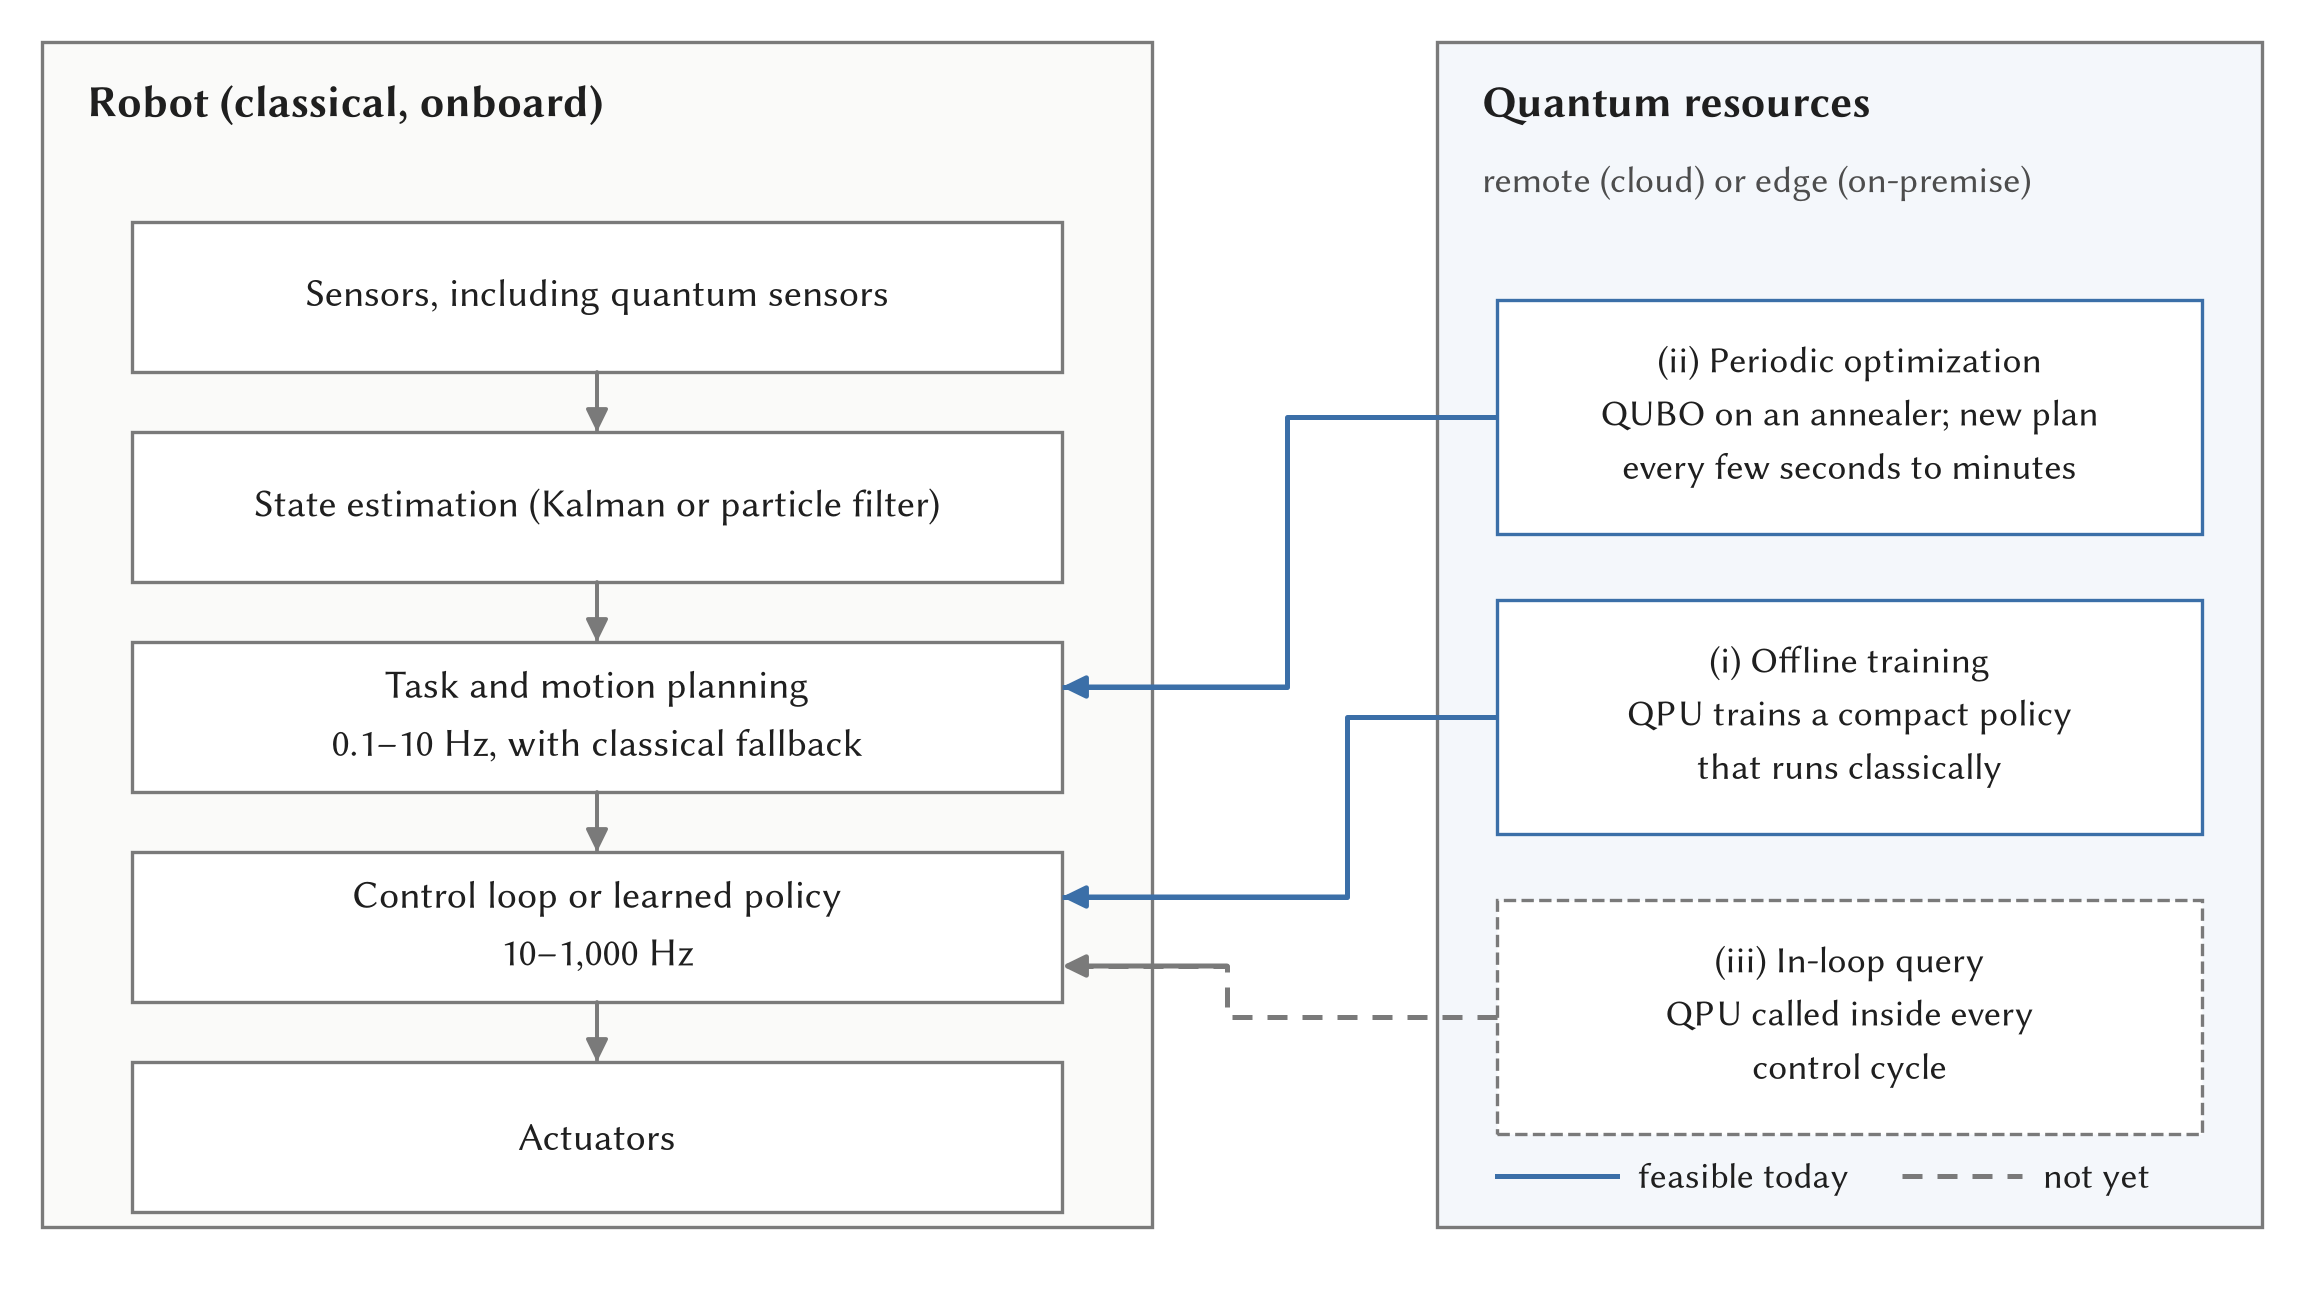
\includegraphics[width=0.95\linewidth]{figures/fig4_architecture.png}
\caption{Positions of quantum resources relative to a robot's classical control stack. Offline training (i) and periodic, asynchronous optimization with a classical fallback (ii) are feasible today; an in-loop quantum query (iii) is not.}
\Description{Block diagram of a robot's classical sense-plan-act stack with a fast control loop, connected to a quantum processor in three ways: (i) offline training producing a classical policy, (ii) asynchronous periodic optimization with a classical fallback, and (iii) a run-time query inside the control loop, marked as not feasible today.}
\label{fig:architecture}
\end{figure}

\paragraph{Deployment models.} Current superconducting processors require dilution refrigerators~\cite{Kjaergaard2020}, so robots access QPUs through the cloud (IBM Quantum, Amazon Braket, and D-Wave Leap), as in qRobot's Raspberry-Pi-based controller~\cite{AtchadeAdelomou2021}. In the medium term, the realistic model is an \emph{edge} deployment, an on-premise QPU serving a factory or warehouse fleet, in line with the wider move to couple QPUs tightly with high-performance computing centers~\cite{Dobler2025}. An onboard QPU on a mobile robot, as \citet{Benioff1998} and \citet{Dong2006} imagined it, is out of reach with present technology~\cite{Mannone2025}.

\paragraph{Execution modes.} Batch execution, such as offline training or overnight planning, tolerates any latency. Asynchronous execution, in which a QPU refines a plan while a classical fallback keeps the robot running, tolerates seconds to minutes. Real-time execution, with a QPU call inside a millisecond control cycle, is not possible today.

\paragraph{Architecture patterns.} Three patterns recur: classical candidate generation followed by quantum selection, in which candidate paths are generated classically and their combination is chosen by annealing~\cite{Clark2019,Ohzeki2019}; quantum function approximation within classical RL loops~\cite{Hohenfeld2024,Dragan2025}; and quantum sensing fused with classical estimation~\cite{Cheiney2018}. Newer capabilities extend these patterns. Dynamic circuits with mid-circuit measurement and real-time classical feed-forward~\cite{Corcoles2021} bring classical decision logic inside a quantum computation, which closed-loop use will require. Circuit cutting~\cite{Tang2021} spreads large circuits across several small QPUs and reconstructs the result classically. Error-mitigated variational pipelines~\cite{Endo2021} and CVaR objectives~\cite{Barkoutsos2020} improve solution quality per shot.


\subsection{Hardware Constraints}\label{sec:hardware}
\paragraph{Platforms and qubit counts.} Superconducting processors lead in qubit count and gate speed but require millikelvin cryogenics~\cite{Kjaergaard2020}; trapped-ion devices offer higher fidelities and all-to-all connectivity at slower gate speeds, as used by \citet{Widdows2023}; and photonic and annealing platforms serve specialized workloads~\cite{Peruzzo2014,Johnson2011}. It is striking how small the robotics circuits are. Gate-based experiments used one to eight qubits, even on processors with up to 64~\cite{Otani2025,Altrabulsi2026,Innan2025}, whereas annealer studies solved QUBOs for up to 200 robots directly~\cite{Clark2019} and for 1,000-AGV fleets only after decomposition into subproblems below 10,000 variables~\cite{Quang2025}.

\paragraph{Noise, mitigation, and fault tolerance.} Gate errors and decoherence limit circuit depth~\cite{Preskill2018}. Error mitigation, including zero-noise extrapolation and probabilistic error cancellation~\cite{Temme2017}, improves expectation values on real processors~\cite{Kandala2019}, but its sampling overhead grows exponentially with circuit size~\cite{Cai2023}. In robotics, noise degraded localization accuracy on real devices~\cite{Antero2025} and training in noisy simulation~\cite{Sinha2023}. Algorithms with provable speed-ups need logical qubits protected by error correction~\cite{Terhal2015}. At realistic error rates, surface codes need on the order of a thousand physical qubits per logical qubit~\cite{Fowler2012}. Low-density parity-check codes cut this by about an order of magnitude~\cite{Bravyi2024}, and below-threshold operation has now been demonstrated~\cite{GoogleQAI2025}. Even so, resource estimates for industrially useful chemistry already call for large fault-tolerant machines running for a long time~\cite{Reiher2017,Kim2022}.

\paragraph{Latency and cloud access.} Analysis of two years of IBM Quantum cloud usage found queueing times ranging from under a minute to over days and a threefold variation in fidelity across machines~\cite{Ravi2021}. A D-Wave anneal takes microseconds~\cite{Ohzeki2019}. The end-to-end latency, with network access, embedding, and post-processing, is far longer, and robotics studies rarely report it. The only study that reported it measured 10,110 s for a workflow that a classical solver finished in 0.03 s~\cite{Willmann2025}.

\paragraph{Quantum-classical communication and resources.} Variational algorithms require many iterations of circuit execution, measurement, and classical update~\cite{McClean2016}, each crossing the quantum-classical boundary. Data encoding costs circuit depth too. HHL-type speed-ups presuppose efficient state preparation and allow only limited read-out~\cite{Harrow2009,Aaronson2015}, and high-dimensional robot observations have to be compressed before encoding~\cite{Chen2022}. Estimating an expectation value to precision $\epsilon$ takes $O(1/\epsilon^2)$ shots, multiplied by the mitigation overhead~\cite{Cai2023} and by the number of optimizer iterations. On the simulation side, the robotics circuits hit classical memory limits at about 27--40 qubits~\cite{Chella2022,Antero2025}.

\paragraph{Size, weight, power, and cooling.} Cryogenic quantum computers cannot be carried by mobile robots~\cite{Kjaergaard2020,Mannone2025}, and cold-atom sensors still need substantial SWaP reductions~\cite{Bongs2019}.

\paragraph{Evidence level.} Hybrid architectures are demonstrated at L3, and at L4 only in simulation-coupled settings, such as Webots-Qiskit swarms~\cite{Mannone2025} and CARLA~\cite{Sinha2023}. Two cart-pole studies give the first measured latency budgets. A cloud QPU took seconds per decision where the control loop needed milliseconds~\cite{Sun2025}, and direct programming of the control electronics sped up on-premise execution by more than an order of magnitude without yet reaching closed-loop rates~\cite{Ngo2026}.

\paragraph{The latency problem.} More and better qubits will not solve this on their own. A shared, cryogenic processor reached over a network cannot sit inside a millisecond control loop, so the constraint is architectural as much as technological. For the near term, the most promising architecture keeps the QPU out of the real-time loop and uses it for training, for periodic fleet-level optimization with a classical fallback, or for sensing.


\section{Quantum Cognition for Robot Decision-Making}\label{sec:cognition}

\subsection{Motivation and Formalism}\label{sec:cog-formalism}
More and more, robots make decisions with people and about people, and people do not reason by the rules of classical (Bayesian) probability. Question-order effects, conjunction and disjunction fallacies, and violations of the sure-thing principle are well documented~\cite{Pothos2013}. Classical robot decision-making relies on Markov decision processes and POMDPs~\cite{Kaelbling1998,Kurniawati2022} and on dynamic stochastic models of choice such as decision field theory~\cite{Busemeyer1993}, all of which assume classical, context-independent probabilities. Quantum cognition offers a different formalism, and it needs neither a quantum computer nor a ``quantum brain''. In quantum probability (QP), beliefs are unit vectors in a Hilbert space, propositions are subspaces, and judgments are projections~\cite{Busemeyer2012}. Probabilities are squared lengths of projections, so the order of sequential judgments matters because projectors need not commute,

\begin{equation}
\Pr(A\text{ then }B)=\lVert P_B P_A\psi\rVert^2 \neq \lVert P_A P_B\psi\rVert^2=\Pr(B\text{ then }A),
\end{equation}
and interference terms can make the probability of a disjunction lower than that of either component. These properties reproduce the empirical violations with few parameters~\cite{Pothos2013,Pothos2022}. A cognitive state can stay indefinite with respect to a judgment until a decision is required. Composite judgments can be entangled, which represents concept combinations that cannot be decomposed~\cite{Busemeyer2012}. And contextuality, the dependence of an outcome on the other measurements made with it, explains why the order and framing of information change decisions~\cite{Pothos2022}. This is what makes the formalism interesting for robots. It can model how the order of a robot's own observations, questions, or recommendations shifts what a human partner is likely to answer, something classical POMDP observation models do not capture. Supplementary Figure S5 gives the geometric picture behind the question-order effect.



\subsection{Robotic and Human-Machine Applications}\label{sec:cog-apps}
\citet{Widdows2023} showed that several QP models of human decision-making can be implemented directly as circuits on quantum hardware: mental states are represented in qubit registers, and judgments correspond to gates and projective measurements. With reusable circuit components for question-order effects and decisions under uncertainty, experiments on an 11-qubit IonQ trapped-ion computer showed that very small circuits, some with a single qubit, reproduce well-documented non-classical patterns of human judgment. The authors are careful to claim neither that the brain uses qubits nor any computational advantage, since models this small are easy to simulate classically. What robotics gains is a set of building blocks for putting QP models into a robot's decision module, for example to predict human responses in human-robot interaction (HRI). \citet{Yan2021} proposed ``quantum affective computing''. A robot's emotion is a superposition over basis emotions in a qubit-encoded emotion space, unitary operators model the transitions between emotional states, and the emotions of communicating robots are fused through entanglement, which saves qubits and gates when representing a whole group. It has been shown only in small simulations, not against human emotional data.

\citet{DeCarolis2025} reviewed more than 35 studies published between 2021 and 2025 on quantum computing for social robotics, as groundwork for a project on quantum-enhanced HRI. They proposed recasting HRI problems such as emotion recognition, path finding, and cognitive modeling as quantum search or QML problems, without yet reporting an implementation. \citet{Daglarli2025} integrated quantum routines (Deutsch-Jozsa, Bernstein-Vazirani, and Grover search) into a brain-inspired cognitive architecture for autonomous agents that combines a prefrontal-cortex-inspired model, transformer-based RL, metacognition, and situation awareness. In a Minecraft-based simulation, the quantum-enhanced agent reached an 80\% success rate about twice as fast as its classical counterpart and collected about 15\% more cumulative reward. The circuits were simulated, however, and the contribution of each routine is not isolated.

Quantum-like models have also been proposed for human-machine teams, the setting in which robots increasingly operate. \citet{Lawless2023} reviewed a quantum-like theory of interdependence for autonomous human-machine teams, arguing that team members' states are non-separable, analogous to entanglement, so that aggregating individual measurements cannot predict team performance. \citet{Humr2025} argued that QP can improve human-AI decision-making by modeling how people rationalize AI outputs: order effects, interference, and ``ontic'' indecision produce belief dynamics that classical probability cannot capture. Although framed for AI decision support, the approach transfers directly to HRI, where a robot's recommendations shape a human partner's judgments. The only decision-making study set on a vehicle task is \citet{Essalmi2026}. Their multi-player quantum game model for automated driving lets each vehicle hold superposed and entangled strategies. In simulated interactive scenarios it raised success rates and reduced collisions compared with classical game-theoretic models, but it has not yet been tested with human drivers or on a real vehicle.

\paragraph{Maturity.} The evidence for QP models of human judgment is extensive and experimentally tested~\cite{Pothos2022}. Their robotic use, by contrast, is at L1--L3: small circuits on an 11-qubit trapped-ion computer~\cite{Widdows2023}, simulated multi-robot emotion fusion~\cite{Yan2021}, a quantum-enhanced cognitive architecture in a game simulation~\cite{Daglarli2025}, a quantum game model for simulated driving interactions~\cite{Essalmi2026}, theoretical models of human-machine teams~\cite{Lawless2023} and human-AI decisions~\cite{Humr2025}, and a project-level agenda for social robots~\cite{DeCarolis2025}.

\paragraph{What is missing.} No study has yet tested a QP-based robot decision module against a classical baseline with human participants. There is an irony here. QP models are small and run classically or on current QPUs, so this branch needs less quantum hardware than any other in the survey, and yet it is the least tested on robots. That it could be deployed today remains a hypothesis until someone runs the experiment with people.


\section{Emerging Directions}\label{sec:emerging}
Five smaller directions are reviewed in full in the supplementary material. \emph{Quantum-inspired robotics} supplies most of the quantum-labeled computational results that have been validated physically: quantum-inspired reinforcement learning on a real robot (L5)~\cite{Dong2012} and particle-swarm SLAM on a real outdoor dataset~\cite{Zuo2018}, both on classical hardware. \emph{Quantum swarm robotics} remains at L1--L4 with toy swarms of up to 10 robots, and its main barrier is that every robot would need QPU access at every interaction step~\cite{Mannone2025}. \emph{Distributed quantum robotics} is at L1--L2. \emph{Quantum computer vision} solves registration and tracking subproblems on annealers (L2--L3 on our scale) but has not been tested on robot data. \emph{Quantum simulation of materials} may help robots indirectly through better batteries and sensors, but industrially relevant problems need large fault-tolerant machines.


\section{Cross-Cutting Analysis}\label{sec:analysis}

\subsection{Synthesis across Robotic Functions}\label{sec:synthesis}
Supplementary Table S7 brings the results together by robotic function. Each function is served by a different quantum paradigm, and the paradigms are at very different stages. Sensing and communication have been fielded on moving platforms, optimization has reached QPU experiments at fleet scale, and learning and planning are still mostly simulated. One pattern stood out to us: the most mature ``quantum'' results in computation are quantum-inspired and run on classical hardware~\cite{Dong2012,Zuo2018}. We did not find a genuinely quantum computational result that is both large enough to be classically hard and better than a properly sized classical baseline~\cite{Hohenfeld2024,Dragan2025,Ohzeki2019,Leib2023}.



\subsection{Evidence Hierarchy}\label{sec:hierarchy}
Figure \ref{fig:evidence} places the 65 empirical and theoretical primary studies (the 7 reviews are excluded) on the evidence hierarchy of Table \ref{tab:levels}. Most of the weight sits at the bottom: 6 studies are at L1, 19 at L2, 23 at L3, and 10 at L4, all of the latter in simulated robot environments. At L5, quantum communication has been demonstrated on drones, vehicles, and cooperating robots~\cite{Tian2023,Conrad2025,Khoshnoud2020,Liu2021}, one quantum-inspired learning method has run on a physical robot~\cite{Dong2012}, and one simulated variational policy has balanced a physical cart-pole~\cite{Sun2025}, giving six studies at that level. Only one quantum technology, magnetic-anomaly navigation with quantum magnetometers, has reached end-to-end field deployment with a measured advantage over a classical baseline (L6)~\cite{Muradoglu2025}. No genuinely quantum computational method has run on a QPU while controlling a physical system; the one that reached L5 executes its circuit in classical simulation~\cite{Sun2025}. We should also be honest about the single L6 rating. It rests on a company-led preprint, and the airborne trials used a crewed aircraft, not an uncrewed robot~\cite{Muradoglu2025}. Discount it, and no study in the corpus goes beyond L5. The ranking of the branches would stay the same, because quantum communication would still be fielded on moving robots, but the claim that quantum sensing has improved navigation in the field would then rest on laboratory and simulation evidence alone~\cite{Cheiney2018,Wang2021,Wang2023}.

Table \ref{tab:execution} adds the quantum-execution tag to this picture. Only 22 of the 65 studies ran any part of their quantum computation on a quantum processor, and 21 of them sit at L3. The ten L4 studies are robot-in-the-loop only in simulation, and nine of them also simulate their quantum circuits; the one exception routes subproblems of a simulated 1,000-AGV fleet to a D-Wave annealer~\cite{Quang2025}. An L4 rating therefore means realistic robot integration, not stronger quantum evidence than L3, and the level and the tag need to be read together. Table \ref{tab:qpu} looks more closely at the 22 studies that did use a quantum processor. Two things stand out. The instances run on the hardware are small, from one qubit to a few thousand annealer variables, and the large fleets reach the device only as decomposed subproblems~\cite{Quang2025}. And only six of the 22 compared against a mature classical method, a commercial solver or a state-of-the-art planner~\cite{Ohzeki2019,Smierzchalski2024,Leib2023,Willmann2025,Osaba2025,Gerlach2025}. Only two of the six report an edge over the classical side, one in a short paper with a proprietary hybrid solver~\cite{Osaba2025} and one in which the quantum or quantum-inspired solver handles small subproblems inside a classical optimal framework~\cite{Gerlach2025}; in neither is the gain attributable to the quantum processor alone.


\begin{table}[tbp]
\caption{Evidence level (rows) by where the quantum component was executed (columns) for the 65 primary studies (7 reviews excluded). ``Simulated'' includes two studies of simulated quantum sensors~\cite{Wang2021,Wang2023}; HW = hardware; QI = quantum-inspired algorithms on conventional hardware.}
\label{tab:execution}
\footnotesize
\begin{tabular}{@{}lrrrrrr@{}}
\toprule
\textbf{Level} & \textbf{None} & \textbf{Simulated} & \textbf{QPU} & \textbf{Sensor/link HW} & \textbf{Classical (QI)} & \textbf{Total} \\ \midrule
L1 Theoretical & 6 & -- & -- & -- & -- & 6 \\
L2 Simulation & -- & 17 & -- & -- & 2 & 19 \\
L3 QPU experiment & -- & -- & 21 & 2 & -- & 23 \\
L4 Robot-in-the-loop & -- & 9 & 1 & -- & -- & 10 \\
L5 Physical demonstration & -- & 1 & -- & 4 & 1 & 6 \\
L6 End-to-end deployment & -- & -- & -- & 1 & -- & 1 \\ \midrule
Total & 6 & 27 & 22 & 7 & 3 & 65 \\
\bottomrule
\end{tabular}
\end{table}

\begin{table}[tbp]
\caption{The 22 primary studies that ran part of their quantum computation on a quantum processor: device, the largest instance run on it, the strongest classical baseline, and the outcome. -- = no classical comparison recorded in our extraction; DA = Fujitsu Digital Annealer; MCL = Monte Carlo localization.}
\label{tab:qpu}
\scriptsize
\begin{tabular}{@{}>{\raggedright\arraybackslash}p{0.170\dimexpr\linewidth-10\tabcolsep\relax}>{\raggedright\arraybackslash}p{0.150\dimexpr\linewidth-10\tabcolsep\relax}>{\raggedright\arraybackslash}p{0.230\dimexpr\linewidth-10\tabcolsep\relax}>{\raggedright\arraybackslash}p{0.190\dimexpr\linewidth-10\tabcolsep\relax}>{\raggedright\arraybackslash}p{0.260\dimexpr\linewidth-10\tabcolsep\relax}@{}}
\toprule
\textbf{Study} & \textbf{Device} & \textbf{Largest instance on the QPU} & \textbf{Strongest baseline} & \textbf{Outcome} \\ \midrule
\citet{Clark2019} & D-Wave 2000Q & Up to 200 robots on a grid & Classical benchmark runs & Valid plans; anneal time only \\
\citet{Ohzeki2019} & D-Wave 2000Q & 10 AGVs, $\le$60 variables & Gurobi; Digital Annealer & Classical and DA handle larger instances \\
\citet{Quang2025} & D-Wave & Sub-QUBOs ($<$10,000 variables) of a 1,000-AGV fleet & -- & No quantum-vs-classical comparison \\
\citet{Smierzchalski2024} & D-Wave hybrid & 21 AGVs ($\approx$1,300 variables) & CPLEX & Comparable \\
\citet{Leib2023} & D-Wave hybrid & Laboratory transport scheduling & Gurobi; Digital Annealer & Gurobi 10--100$\times$ faster on small; DA best on largest \\
\citet{Schuetz2022} & D-Wave (Braket) & Reduced sub-problems & Classical BRKGA & Performance from classical algorithm \\
\citet{Willmann2025} & D-Wave Advantage 4.1 & 4 tasks, 2 workstations & Exact classical solver & 10,110 s vs.\ 0.03 s end to end \\
\citet{Osaba2025} & D-Wave hybrid & 5 inspection cases & Gurobi; OR-Tools & Competitive quality, less time (preliminary) \\
\citet{AtchadeAdelomou2021} & IBM, Braket, D-Wave & Small warehouse instances & -- & Valid routes \\
\citet{Windmann2023} & IBM Q System One & Small AS/RS instances & -- & Only small instances fit \\
\citet{Salloum2026} & D-Wave Pegasus, Zephyr & Two-link planar IK & Classical QUBO solvers & Lower time-to-solution on larger instances; not better than continuous IK \\
\citet{Otani2025} & RIKEN/Fujitsu 64-qubit & 2 qubits & -- & Entanglement helps vs.\ no-entanglement circuit \\
\citet{Goncalves2018} & IBM 5-qubit & A few qubits & -- & Feasibility only \\
\citet{Gerlach2025} & D-Wave Advantage & Small QUBO subproblems in BCP & BCP, EECBS, LaCAM*, LNS2 & Competitive with state of the art \\
\citet{Innan2025} & IBM ibm\_kyiv & Small flight graphs & -- & Feasible paths despite noise \\
\citet{OsabaDrone2025} & D-Wave & 3 drone-routing cases & -- & Feasible routes \\
\citet{Antero2025} & IBM Brisbane (127-qubit); IonQ noise model & Small 2D grid maps & MCL (analytical) & Accuracy falls as maps grow \\
\citet{Altrabulsi2026} & IBM ibm\_fez & Trained 8-qubit policy & Tabular Q, MLP, SNN (sim.) & Hardware run as feasibility check \\
\citet{Ngo2026} & VTT Q5 & 1-qubit agent & -- & $>$10$\times$ faster execution, below control rate \\
\citet{Widdows2023} & IonQ 11-qubit & 1 to a few qubits & n/a & Reproduces judgment patterns \\
\citet{Mannone2022} & IBM & 4-qubit swarm model & -- & Toy model \\
\citet{Mannone2023} & IBM & Swarms of 3 and 10 robots & -- & Modeling only \\
\bottomrule
\end{tabular}
\end{table}

\begin{figure}[t]
\centering
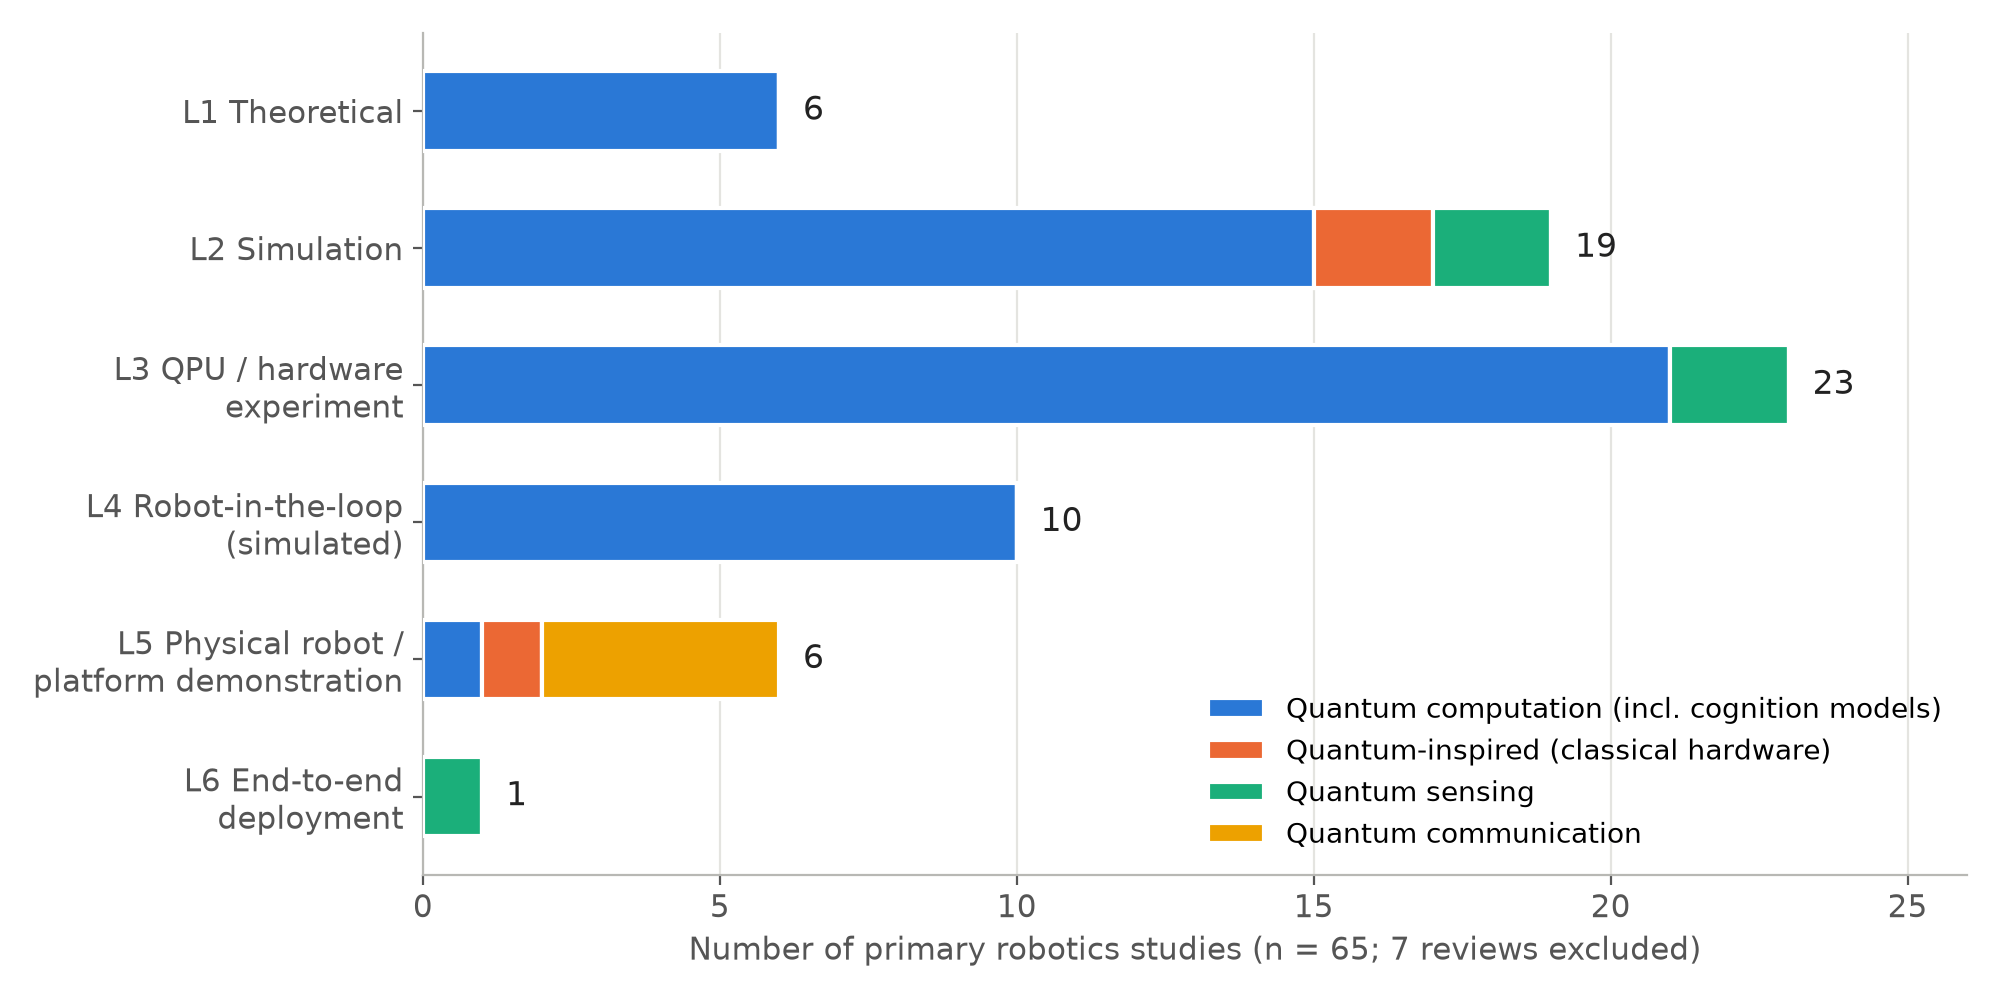
\includegraphics[width=0.90\linewidth]{figures/fig2_evidence.png}
\caption{Evidence levels reached by the 65 primary robotics studies (7 reviews excluded), by technology type. The only quantum computational study at L5 runs its circuit in classical simulation on a physical cart-pole; the other studies at L5 and L6 use quantum sensing, quantum communication, or quantum-inspired classical computation.}
\Description{Stacked horizontal bar chart of the number of studies at each evidence level from L1 to L6, colored by technology type (quantum computation including quantum-probability models, quantum-inspired classical computation, quantum sensing, and quantum communication); most studies are at L2 and L3; L5 holds one simulated quantum policy on a physical cart-pole, one quantum-inspired study, and four quantum-communication studies, and L6 holds one quantum-sensing study.}
\label{fig:evidence}
\end{figure}


\subsection{Claims of Quantum Advantage versus Evidence}\label{sec:claims}
Claims of quantum advantage in the robotics literature refer to four different things, which should not be confused.

\paragraph{Theoretical speed-up.} Provable speed-ups relevant to robotics are quadratic for search, amplitude estimation, and Monte Carlo sampling~\cite{Grover1996,Brassard2002,Montanaro2015}, and exponential only for structured problems such as linear systems under strong input/output assumptions~\cite{Harrow2009,Aaronson2015}. Dequantization has since weakened many of these~\cite{Tang2019,Chia2020}. For NP-hard optimization there is no provable advantage~\cite{Farhi2014}, and a provable learning separation for quantum policies exists only for artificial tasks built on the discrete logarithm~\cite{Jerbi2021}.

\paragraph{Simulated speed-up.} Simulated studies usually report fewer iterations, oracle queries, or parameters, not lower wall-clock time: $O(\sqrt{N})$ query counts for localization~\cite{Antero2025} and planning~\cite{Chella2022}, faster swarm convergence against generic ant simulations~\cite{Chella2023}, and parameter reductions of about 100--200 times in QRL~\cite{Acuto2022,Dragan2025}. None of these metrics accounts for circuit depth, shots, error mitigation, or the cost of classical simulation, and the baselines are rarely state of the art.

\paragraph{Hardware demonstration.} Hardware demonstrations show that something can be done, not that it is better. The list is longer than one might expect: valid annealer plans for up to 200 robots~\cite{Clark2019}, collision-free AGV control~\cite{Ohzeki2019}, decomposed routing of a 1,000-AGV fleet~\cite{Quang2025}, optimal MAPF with QUBO subproblems~\cite{Gerlach2025}, QAOA drone paths on IBM hardware~\cite{Innan2025}, annealer-based IK~\cite{Salloum2026}, two-qubit kinematics on a 64-qubit processor~\cite{Otani2025}, storage-and-retrieval scheduling with QAOA~\cite{Windmann2023}, drone routing on annealers~\cite{OsabaDrone2025}, a single-qubit control agent on a superconducting QPU~\cite{Ngo2026}, a navigation policy executed on IBM hardware~\cite{Altrabulsi2026}, and cognitive circuits on trapped ions~\cite{Widdows2023}. Wherever a comparison was made, classical solvers stayed competitive or did better~\cite{Ohzeki2019,Smierzchalski2024,Leib2023,Willmann2025}. The advantages on the largest instances came from quantum-inspired digital hardware~\cite{Leib2023}, and hardware noise cost accuracy~\cite{Antero2025}.

\paragraph{End-to-end robotics advantage.} Better task performance in a realistic robotic deployment against a strong classical baseline has been shown only for quantum sensing~\cite{Muradoglu2025}. Quantum communication has been deployed between moving platforms~\cite{Conrad2025}, but it offers security rather than a performance advantage. For quantum computation, nobody has yet shown an end-to-end advantage on a robot.


\subsection{The Latency Gap}\label{sec:latency}
Figure \ref{fig:latency} compares the relevant timescales. Robot control loops run at 10--1,000 Hz and planning loops at roughly 0.1--10 Hz, whereas cloud QPU access involves queueing from under a minute to several days~\cite{Ravi2021}, on top of compilation, embedding, many shots, and post-processing. Variational methods multiply all of this by hundreds of optimizer iterations~\cite{McClean2016}. That leaves only three ways to integrate a QPU today: offline training~\cite{Sinha2023}, asynchronous periodic optimization with a classical fallback~\cite{Ohzeki2019}, and sensing~\cite{Muradoglu2025}. Dynamic circuits~\cite{Corcoles2021} and on-premise edge QPUs may shorten latency in the future, but real-time quantum control of robots is not around the corner.

\begin{figure}[t]
\centering
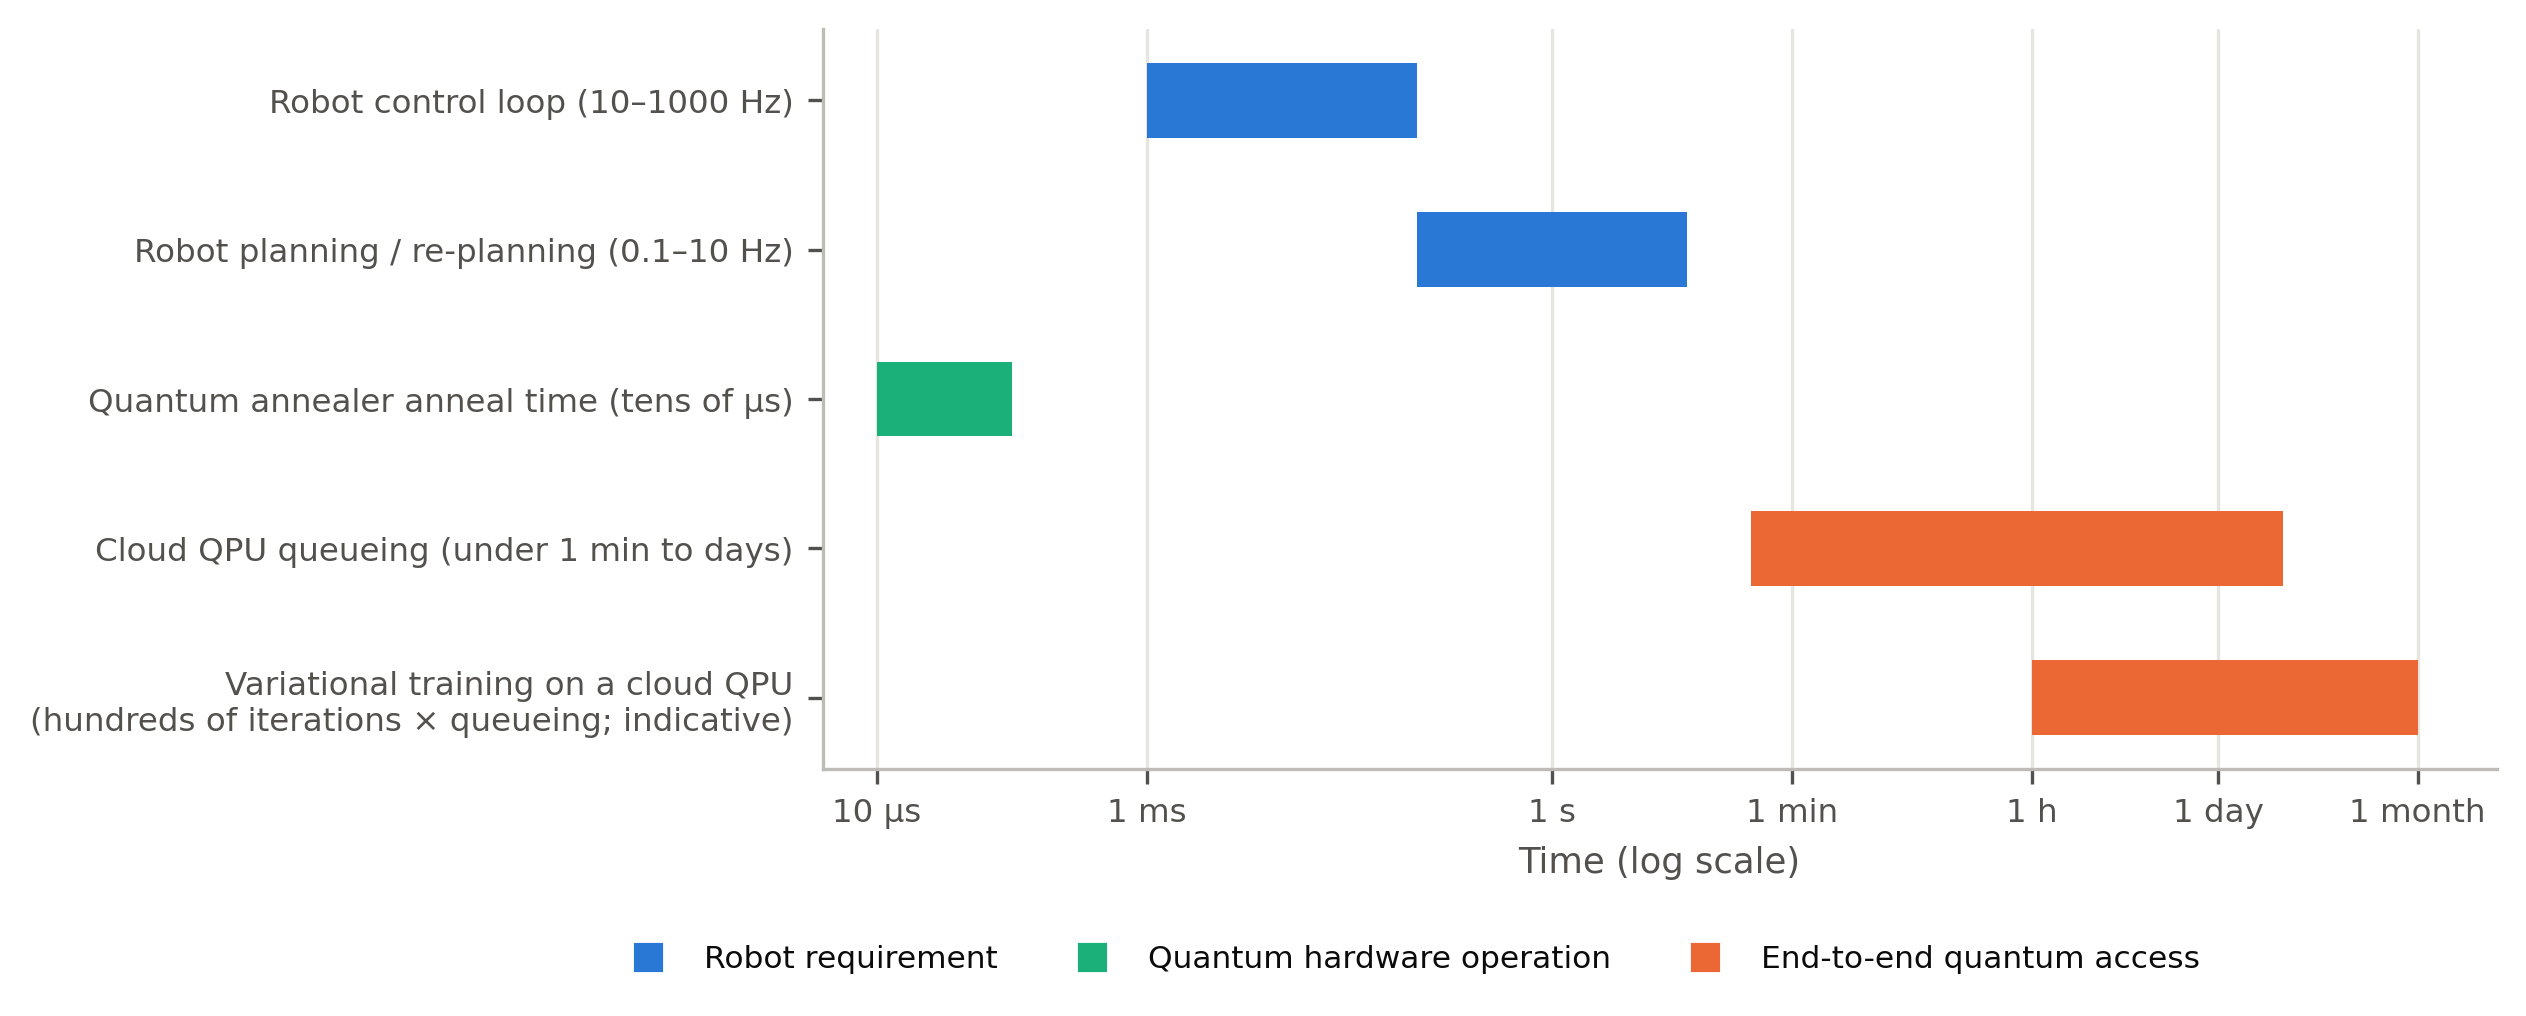
\includegraphics[width=0.92\linewidth]{figures/fig5_latency.png}
\caption{Timescales of robot control and planning compared with quantum hardware operation and end-to-end cloud quantum access (log scale). The anneal time is from \citet{Ohzeki2019} and the queueing range from \citet{Ravi2021}; the range for variational training is indicative.}
\Description{Log-scale horizontal chart of timescales from microseconds to days: gate and anneal times in microseconds, robot control loops at 1 to 100 milliseconds, planning loops at 0.1 to 10 seconds, variational training in minutes to hours, and cloud queueing from about a minute to several days.}
\label{fig:latency}
\end{figure}


\subsection{Scalability}\label{sec:scalability}
Scaling runs into limits on four fronts. QAOA needs hundreds to thousands of qubits before any advantage appears~\cite{Guerreschi2019}. Barren plateaus limit trainability~\cite{McClean2018,Larocca2025}. Robot sensor data must be compressed before it can be encoded~\cite{Chen2022}. And results become hard to verify, because classical simulation of the circuits used in robotics stops at about 27--40 qubits~\cite{Chella2022,Antero2025}. So far the robotics studies have stayed at toy scale: grid worlds, swarms of up to 10 robots, two-link manipulators. The hardware adds its own limits: noise and decoherence~\cite{Preskill2018}, exponential error-mitigation overheads~\cite{Cai2023}, fault-tolerance overheads of hundreds to about a thousand physical qubits per logical qubit~\cite{Fowler2012,Bravyi2024}, cryogenic SWaP-C~\cite{Kjaergaard2020}, restricted annealer connectivity, and the bandwidth, dynamic-range, and size limits of quantum sensors~\cite{Bongs2019,Wang2021}.


\subsection{A Worked Resource Estimate}\label{sec:resource}
Several studies in this survey rest their case on a quadratic speed-up that would need fault-tolerant hardware. To see what such a speed-up would buy a robot, we made a rough estimate for the clearest example, Grover-based localization on a known map~\cite{Antero2025}. The numbers are ours and deliberately generous to the quantum side; Table \ref{tab:resource} lists the assumptions.

Take a $1{,}000\times 1{,}000$ occupancy grid, $N=10^6$ cells, which at 5 cm resolution covers a $50\times 50$ m floor. Grover search needs about $\frac{\pi}{4}\sqrt{N}\approx 785$ iterations. Each iteration calls the oracle, and the oracle must read the map: without quantum random-access memory, which does not exist as hardware, the standard way to load $N$ classical entries into a circuit costs about $4N$ T gates, or roughly $N$ Toffoli gates, per call~\cite{Babbush2018}, or about $2N$ when the call is also uncomputed. At $10~\mu$s per error-corrected Toffoli gate, about 17 times faster than the $170~\mu$s that \citet{Babbush2021} estimate for a surface-code machine, the search takes about $785\times 2\times 10^6\times 10~\mu\mathrm{s}\approx 1.6\times 10^4$ s, roughly four and a half hours. A classical scan of the same map, at 10 ns per cell, takes 10 ms. The quantum search therefore loses by six orders of magnitude, because loading the map costs as much as the classical search it was meant to replace.

Suppose instead that a qRAM with logarithmic access time existed, so that each oracle call cost only $10^3$ Toffoli gates. The search would then take about 16 s, still far slower than the 10 ms classical scan and far outside a localization loop that runs at several hertz. Under these assumptions the two methods break even only for maps of about $2.5\times 10^{12}$ cells, where each search takes about seven hours. The machine itself would need on the order of 170 logical qubits for the address, pattern, and comparison registers, or a few hundred thousand physical qubits at surface-code distance 25~\cite{Fowler2012}, before counting the magic-state factories. These figures agree with the general analysis of \citet{Babbush2021}, who argue that quadratic speed-ups are unlikely to give a runtime advantage on early fault-tolerant machines. The estimate is crude, and better circuits would shift the numbers, but not by the six orders of magnitude needed to change the conclusion.

\begin{table}[tbp]
\caption{Assumptions and results of the resource estimate for Grover localization (Section \ref{sec:resource}). All values are order-of-magnitude estimates chosen to favor the quantum method.}
\label{tab:resource}
\footnotesize
\begin{tabular}{@{}>{\raggedright\arraybackslash}p{0.46\dimexpr\linewidth-4\tabcolsep\relax}>{\raggedright\arraybackslash}p{0.54\dimexpr\linewidth-4\tabcolsep\relax}@{}}
\toprule
\textbf{Quantity} & \textbf{Value} \\ \midrule
Map size $N$ & $10^6$ cells ($1{,}000\times 1{,}000$ grid) \\
Grover iterations & $\frac{\pi}{4}\sqrt{N}\approx 785$ \\
Oracle cost, map loaded by table lookup & $\approx 2N$ Toffoli gates per iteration~\cite{Babbush2018} \\
Oracle cost, hypothetical log-time qRAM & $\approx 10^3$ Toffoli gates per iteration \\
Error-corrected Toffoli time & 10 $\mu$s (vs.\ $\approx$170 $\mu$s estimated by \citet{Babbush2021}) \\
Classical scan & 10 ns per cell, 10 ms per map \\
Quantum time, table lookup & $\approx 1.6\times 10^4$ s (about 4.4 h) \\
Quantum time, with qRAM & $\approx 16$ s \\
Break-even map size, with qRAM & $\approx 2.5\times 10^{12}$ cells (about 7 h per search) \\
Logical / physical qubits & $\approx 170$ / $\approx 2\times 10^5$ (distance 25), excluding factories \\
\bottomrule
\end{tabular}
\end{table}


\section{Open Challenges and Research Agenda}\label{sec:challenges}
We take the open challenges from the taxonomy of Figure \ref{fig:taxonomy}. For each robotic function we describe the gap between today's evidence and a deployable result, and then turn to the challenges that cut across all functions. Supplementary Table S9 arranges the resulting research directions by time horizon.


\subsection{Challenges by Robotic Function}\label{sec:ch-function}
\paragraph{Optimization.} The open question is whether quantum hardware adds anything to a well-engineered QUBO pipeline. Studies need \emph{instance families} on which quantum, quantum-inspired, and classical solvers are compared on equal end-to-end terms, including embedding and queueing, at the sizes of real fleets~\cite{Leib2023,Quang2025}. Constraint-preserving mixers~\cite{Hadfield2019} have been tested on robot task allocation only in simulation~\cite{Bang2026}, and transferable QAOA parameters~\cite{Zhou2020} not at all. The most promising template, in our view, places small QUBOs inside a provably optimal classical framework~\cite{Gerlach2025}.

\paragraph{Planning.} Grover-based planning and localization need oracle constructions whose qubit counts and depth scale gracefully with map size, and evaluations against A*, RRT*~\cite{Karaman2011}, and Monte Carlo localization~\cite{Dellaert1999} on realistic maps. Our rough estimate in Section \ref{sec:resource} suggests that, for localization at least, the quadratic speed-up does not survive the cost of loading the map into the oracle; a careful estimate by specialists, with optimized circuits, would settle the question for planning as well~\cite{Babbush2021}. A useful first experiment is modest: take one published Grover planner, count its logical resources exactly, and compare the resulting wall-clock time with A* on the same map.

\paragraph{Learning.} The parameter-efficiency hypothesis of QRL~\cite{Hohenfeld2024,Acuto2022} should be tested for what matters on robots: sample efficiency, training wall-clock time, energy, and robustness on physical platforms, with circuits trained on real QPUs rather than in idealized simulation. Encodings for high-dimensional observations that avoid barren plateaus~\cite{Cerezo2021b,Larocca2025} without becoming classically simulable remain open. The cleanest test would fix a robot task and a sample budget, train a quantum and an adequately sized classical policy under the same budget, and report sample efficiency and wall-clock time; a parameter count alone should no longer be accepted as the headline result.

\paragraph{Sensing and communication.} Quantum navigation sensors need independent field replication~\cite{Muradoglu2025}, miniaturization to the SWaP budgets of small robots~\cite{Bongs2019}, and integration into standard estimation stacks through Kalman-type fusion~\cite{Cheiney2018,Wang2021}. QKD between robots needs evaluations of range, weather, and alignment under realistic mission profiles~\cite{Conrad2025}. The decisive experiment for navigation is a GNSS-denied mission flown by an uncrewed robot, with the quantum fix inside its own estimator and the same mission flown with a classical INS for comparison; for communication, it is a coordination task whose commands are authenticated with quantum-distributed keys.

\paragraph{Decision-making.} The clearest near-term gap is a QP-based decision and human-modeling layer for robots, evaluated with human participants against Bayesian and POMDP baselines~\cite{Kurniawati2022,Pothos2022}. Such a layer needs little or no quantum hardware~\cite{Widdows2023} and addresses a genuine need in HRI and human-machine teaming~\cite{Lawless2023,Humr2025}. A first study could be small: a robot that asks two questions in either order, a QP model and a Bayesian model fitted to the same participants, and a comparison of how well each predicts the answers to held-out question orders.

\paragraph{Foundation models and physical AI.} Robot learning is moving toward large pretrained models that reason over language and perception, often called physical or embodied AI. In our corpus, quantum methods touch this trend only at the edges: \citet{Bang2026} used a language front end to generate QUBO task assignments, and QRL~\cite{Hohenfeld2024,Acuto2022} and QP decision models~\cite{Pothos2022} address small parts of policy learning and reasoning. No study applied a quantum method to the training or inference of a robot foundation model, so this direction has no graded evidence yet. The obstacles are clear from the rest of this survey: such models have billions of parameters, today's processors offer hundreds of noisy qubits, loading classical data into quantum states can cancel any speed-up~\cite{Aaronson2015}, and dequantization removes several claimed advantages~\cite{Tang2019}. The realistic near-term role is narrower, with quantum solvers handling well-defined combinatorial subproblems that a foundation model formulates, as in \citet{Bang2026}, and the open question is whether that division of labor beats a classical solver end to end.

\paragraph{Where we would place our bets.} If we had to choose, we would invest first in quantum navigation sensing on uncrewed platforms and in QP models for HRI, because both can be tested now and neither depends on fault-tolerant hardware. Next comes fleet-level optimization, but only in studies that report end-to-end time against the best classical solver, since that is where the case for quantum hardware is currently weakest. We would treat Grover-based planning and real-time quantum control as long-term research, worth pursuing for what they teach about algorithm design but not yet as routes to a better robot.


\subsection{Cross-Cutting Challenges}\label{sec:ch-cross}
\paragraph{Reporting standards and benchmarks.} We would have liked to pool the results quantitatively, but the tasks, metrics, and baselines differ too much. Supplementary Table S8 proposes a minimal reporting checklist for quantum-robotics experiments; shared benchmark suites for fleet scheduling, MAPF, navigation RL, and localization would allow results to be compared across studies. Application-level benchmark frameworks already exist outside robotics. QUARK, for example, includes a robot-path reference problem with quantum and classical solvers~\cite{Finzgar2022}, and extending such frameworks to the tasks in this survey would be a direct way to meet the checklist.

\paragraph{Separating quantum from quantum-inspired results.} Quantum-inspired and classical results should be reported separately from quantum-hardware results, and claimed speed-ups should be checked against the best classical algorithm under the same input assumptions~\cite{Aaronson2015,Tang2019}.

\paragraph{Latency-aware architectures.} Architectures should keep the QPU out of the real-time loop, provide classical fallbacks, and report end-to-end latency budgets. Edge QPUs with dynamic circuits~\cite{Corcoles2021} and circuit cutting~\cite{Tang2021} are the main technical routes to closing the latency gap.

\paragraph{Safety and verification.} A robot should not act on a probabilistic quantum output without checking it first. Post-processing that rejects constraint-violating samples~\cite{Ohzeki2019} is a start, but there are no formal guarantees yet for hybrid quantum-classical controllers.



\section{Conclusion}\label{sec:conclusion}
We set out to find what the published evidence says about quantum technologies for robots. After reading 72 primary studies against 107 foundational works, our answer is that quantum robotics is rich in ideas but still early in evidence. Quantum optimization is the most hardware-tested area, from 200-robot routing on annealers to decomposed routing of 1,000-AGV fleets, but classical and quantum-inspired solvers match or beat it in head-to-head comparisons. Quantum search and planning remain simulated. Quantum reinforcement learning reliably reduces parameter counts, but nobody has shown that it produces better or faster policies, and supervised QML faces barren plateaus and dequantization. Quantum sensing is a different story: one field trial, still awaiting independent replication, reports large navigation gains, and QKD already links drones and vehicles in motion. Among the computational results, the ones that have been validated physically are mostly quantum-inspired and run on classical hardware.

For the near term (2026--2030), the realistic opportunities are quantum-enhanced navigation sensing, QP decision models for HRI, offline or periodic QUBO-based fleet optimization with classical fallbacks, and QPU-trained compact policies for embedded deployment. Real-time control will stay classical for the foreseeable future. Until on-premise, low-latency, fault-tolerant processors exist, quantum resources belong outside the millisecond loop, as training accelerators, periodic planners, or sensors. The long-term vision is a hybrid robot in which classical controllers handle real-time control, quantum sensors provide drift-free navigation, remote or edge quantum processors solve fleet-level optimization and train compact policies, and QP models help the robot understand the humans it works with. Getting there will depend less on a single breakthrough than on patient, honest evaluation of each component, on real robots, against the best classical alternative.

\section*{Data Availability}
The data-extraction table for the 72 primary studies, with evidence level, quantum-execution tag, and publication status for each study, the per-study quality appraisal and its criteria, the codebook, the PRISMA 2020 flow diagram and checklist, and the search strings are provided as supplementary material, including machine-readable (CSV) versions of the extraction and appraisal tables.

\bibliographystyle{ACM-Reference-Format}
\bibliography{refs}

\end{document}
